\documentclass[12pt]{article}

%packages
%\usepackage{latexsym}
\usepackage{graphicx}
\usepackage{wrapfig}
\usepackage{color}
\usepackage{amsmath}
\usepackage{dsfont}
\usepackage{placeins}
\usepackage{amssymb}
\usepackage{skull}
\usepackage{enumerate}
\usepackage{soul}
\usepackage{alphalph}
\usepackage{hyperref}
\usepackage{enumerate}
\usepackage{listings}
\usepackage{multicol}
\usepackage{etoolbox}
\usepackage{fancyvrb}
\usepackage{changepage}

%\fancyhf{} % clear all header and footers
%\renewcommand{\headrulewidth}{0pt} % remove the header rule
%\fancyfoot[LE, LO]{\thepage}


%\usepackage{pstricks,pst-node,pst-tree}

%\usepackage{algpseudocode}
%\usepackage{amsthm}
%\usepackage{hyperref}
%\usepackage{mathrsfs}
%\usepackage{amsfonts}
%\usepackage{bbding}
%\usepackage{listings}
%\usepackage{appendix}
\usepackage[margin=1in]{geometry}
%\geometry{papersize={8.5in,11in},total={6.5in,9in}}
\usepackage{cancel}
%\usepackage{algorithmic, algorithm}

\definecolor{dkgreen}{rgb}{0,0.6,0}
\definecolor{gray}{rgb}{0.5,0.5,0.5}
\definecolor{mauve}{rgb}{0.58,0,0.82}
\lstset{ %
  language=R,                     % the language of the code
  basicstyle=\footnotesize,       % the size of the fonts that are used for the code
  numbers=left,                   % where to put the line-numbers
  numberstyle=\tiny\color{gray},  % the style that is used for the line-numbers
  stepnumber=1,                   % the step between two line-numbers. If it's 1, each line
                                  % will be numbered
  numbersep=5pt,                  % how far the line-numbers are from the code
  backgroundcolor=\color{white},  % choose the background color. You must add \usepackage{color}
  showspaces=false,               % show spaces adding particular underscores
  showstringspaces=false,         % underline spaces within strings
  showtabs=false,                 % show tabs within strings adding particular underscores
  frame=single,                   % adds a frame around the code
  rulecolor=\color{black},        % if not set, the frame-color may be changed on line-breaks within not-black text (e.g. commens (green here))
  tabsize=2,                      % sets default tabsize to 2 spaces
  captionpos=b,                   % sets the caption-position to bottom
  breaklines=true,                % sets automatic line breaking
  breakatwhitespace=false,        % sets if automatic breaks should only happen at whitespace
  title=\lstname,                 % show the filename of files included with \lstinputlisting;
                                  % also try caption instead of title
  keywordstyle=\color{black},      % keyword style
  commentstyle=\color{dkgreen},   % comment style
  stringstyle=\color{mauve},      % string literal style
  escapeinside={\%*}{*)},         % if you want to add a comment within your code
  morekeywords={*,...}            % if you want to add more keywords to the set
}

\newcommand{\qu}[1]{``#1''}
\newcommand{\spc}[1]{\\ \vspace{#1cm}}

\newcounter{probnum}
\setcounter{probnum}{1}

%create definition to allow local margin changes
\def\changemargin#1#2{\list{}{\rightmargin#2\leftmargin#1}\item[]}
\let\endchangemargin=\endlist 

%allow equations to span multiple pages
\allowdisplaybreaks

%define colors and color typesetting conveniences
\definecolor{gray}{rgb}{0.5,0.5,0.5}
\definecolor{black}{rgb}{0,0,0}
\definecolor{white}{rgb}{1,1,1}
\definecolor{blue}{rgb}{0.5,0.5,1}
\newcommand{\inblue}[1]{\color{blue}#1 \color{black}}
\definecolor{green}{rgb}{0.133,0.545,0.133}
\newcommand{\ingreen}[1]{\color{green}#1 \color{black}}
\definecolor{yellow}{rgb}{1,0.549,0}
\newcommand{\inyellow}[1]{\color{yellow}#1 \color{black}}
\definecolor{red}{rgb}{1,0.133,0.133}
\newcommand{\inred}[1]{\color{red}#1 \color{black}}
\definecolor{purple}{rgb}{0.58,0,0.827}
\newcommand{\inpurple}[1]{\color{purple}#1 \color{black}}
\definecolor{gray}{rgb}{0.5,0.5,0.5}
\newcommand{\ingray}[1]{\color{gray}#1 \color{black}}
\definecolor{backgcode}{rgb}{0.97,0.97,0.8}
\definecolor{Brown}{cmyk}{0,0.81,1,0.60}
\definecolor{OliveGreen}{cmyk}{0.64,0,0.95,0.40}
\definecolor{CadetBlue}{cmyk}{0.62,0.57,0.23,0}

%define new math operators
\DeclareMathOperator*{\argmax}{arg\,max~}
\DeclareMathOperator*{\argmin}{arg\,min~}
\DeclareMathOperator*{\argsup}{arg\,sup~}
\DeclareMathOperator*{\arginf}{arg\,inf~}
\DeclareMathOperator*{\convolution}{\text{\Huge{$\ast$}}}
\newcommand{\infconv}[2]{\convolution^\infty_{#1 = 1} #2}
%true functions

%%%% GENERAL SHORTCUTS

\makeatletter
\newalphalph{\alphmult}[mult]{\@alph}{26}
\renewcommand{\labelenumi}{(\alphmult{\value{enumi}})}
\renewcommand{\theenumi}{\AlphAlph{\value{enumi}}}
\makeatother
%shortcuts for pure typesetting conveniences
\newcommand{\bv}[1]{\boldsymbol{#1}}

%shortcuts for compound constants
\newcommand{\BetaDistrConst}{\dfrac{\Gamma(\alpha + \beta)}{\Gamma(\alpha)\Gamma(\beta)}}
\newcommand{\NormDistrConst}{\dfrac{1}{\sqrt{2\pi\sigma^2}}}

%shortcuts for conventional symbols
\newcommand{\tsq}{\tau^2}
\newcommand{\tsqh}{\hat{\tau}^2}
\newcommand{\sigsq}{\sigma^2}
\newcommand{\sigsqsq}{\parens{\sigma^2}^2}
\newcommand{\sigsqovern}{\dfrac{\sigsq}{n}}
\newcommand{\tausq}{\tau^2}
\newcommand{\tausqalpha}{\tau^2_\alpha}
\newcommand{\tausqbeta}{\tau^2_\beta}
\newcommand{\tausqsigma}{\tau^2_\sigma}
\newcommand{\betasq}{\beta^2}
\newcommand{\sigsqvec}{\bv{\sigma}^2}
\newcommand{\sigsqhat}{\hat{\sigma}^2}
\newcommand{\sigsqhatmlebayes}{\sigsqhat_{\text{Bayes, MLE}}}
\newcommand{\sigsqhatmle}[1]{\sigsqhat_{#1, \text{MLE}}}
\newcommand{\bSigma}{\bv{\Sigma}}
\newcommand{\bSigmainv}{\bSigma^{-1}}
\newcommand{\thetavec}{\bv{\theta}}
\newcommand{\thetahat}{\hat{\theta}}
\newcommand{\thetahatmm}{\hat{\theta}^{\mathrm{MM}}}
\newcommand{\thetahathatmm}{\thetahathat^{\mathrm{MM}}}
\newcommand{\thetahathatmle}{\thetahathat^{\mathrm{MLE}}}
\newcommand{\thetahatmle}{\hat{\theta}^{\mathrm{MLE}}}
\newcommand{\thetavechatmle}{\hat{\thetavec}^{\mathrm{MLE}}}
\newcommand{\muhat}{\hat{\mu}}
\newcommand{\musq}{\mu^2}
\newcommand{\muvec}{\bv{\mu}}
\newcommand{\muhatmle}{\muhat_{\text{MLE}}}
\newcommand{\lambdahat}{\hat{\lambda}}
\newcommand{\lambdahatmle}{\lambdahat_{\text{MLE}}}
\newcommand{\thetahatmap}{\hat{\theta}_{\mathrm{MAP}}}
\newcommand{\thetahatmmae}{\hat{\theta}_{\mathrm{MMAE}}}
\newcommand{\thetahatmmse}{\hat{\theta}_{\mathrm{MMSE}}}
\newcommand{\etavec}{\bv{\eta}}
\newcommand{\alphavec}{\bv{\alpha}}
\newcommand{\minimaxdec}{\delta^*_{\mathrm{mm}}}
\newcommand{\ybar}{\bar{y}}
\newcommand{\xbar}{\bar{x}}
\newcommand{\Xbar}{\bar{X}}
\newcommand{\iid}{~{\buildrel iid \over \sim}~}
\newcommand{\inddist}{~{\buildrel ind \over \sim}~}
\newcommand{\approxdist}{~{\buildrel \bv{\cdot} \over \sim}~}
\newcommand{\equalsindist}{~{\buildrel d \over =}~}
\newcommand{\loglik}[1]{\ell\parens{#1}}
\newcommand{\thetahatkminone}{\thetahat^{(k-1)}}
\newcommand{\thetahatkplusone}{\thetahat^{(k+1)}}
\newcommand{\thetahatk}{\thetahat^{(k)}}
\newcommand{\half}{\frac{1}{2}}
\newcommand{\third}{\frac{1}{3}}
\newcommand{\twothirds}{\frac{2}{3}}
\newcommand{\fourth}{\frac{1}{4}}
\newcommand{\fifth}{\frac{1}{5}}
\newcommand{\sixth}{\frac{1}{6}}

%shortcuts for vector and matrix notation
\newcommand{\A}{\bv{A}}
\newcommand{\At}{\A^T}
\newcommand{\Ainv}{\inverse{\A}}
\newcommand{\B}{\bv{B}}
\renewcommand{\b}{\bv{b}}
\renewcommand{\H}{\bv{H}}
\newcommand{\K}{\bv{K}}
\newcommand{\Kt}{\K^T}
\newcommand{\Kinv}{\inverse{K}}
\newcommand{\Kinvt}{(\Kinv)^T}
\newcommand{\M}{\bv{M}}
\newcommand{\Bt}{\B^T}
\newcommand{\Q}{\bv{Q}}
\newcommand{\Qt}{\Q^T}
\newcommand{\R}{\bv{R}}
\newcommand{\Rt}{\R^T}
\newcommand{\Z}{\bv{Z}}
\newcommand{\X}{\bv{X}}
\newcommand{\Xsub}{\X_{\text{(sub)}}}
\newcommand{\Xsubadj}{\X_{\text{(sub,adj)}}}
\newcommand{\I}{\bv{I}}
\newcommand{\Y}{\bv{Y}}
\newcommand{\sigsqI}{\sigsq\I}
\renewcommand{\P}{\bv{P}}
\newcommand{\Psub}{\P_{\text{(sub)}}}
\newcommand{\Pt}{\P^T}
\newcommand{\Pii}{P_{ii}}
\newcommand{\Pij}{P_{ij}}
\newcommand{\IminP}{(\I-\P)}
\newcommand{\Xt}{\bv{X}^T}
\newcommand{\XtX}{\Xt\X}
\newcommand{\XtXinv}{\parens{\Xt\X}^{-1}}
\newcommand{\XtXinvXt}{\XtXinv\Xt}
\newcommand{\XXtXinvXt}{\X\XtXinvXt}
\newcommand{\x}{\bv{x}}
\newcommand{\w}{\bv{w}}
\newcommand{\q}{\bv{q}}
\newcommand{\zerovec}{\bv{0}}
\newcommand{\onevec}{\bv{1}}
\newcommand{\oneton}{1, \ldots, n}
\newcommand{\yoneton}{y_1, \ldots, y_n}
\newcommand{\yonetonorder}{y_{(1)}, \ldots, y_{(n)}}
\newcommand{\Yoneton}{Y_1, \ldots, Y_n}
\newcommand{\iinoneton}{i \in \braces{\oneton}}
\newcommand{\onetom}{1, \ldots, m}
\newcommand{\jinonetom}{j \in \braces{\onetom}}
\newcommand{\xoneton}{x_1, \ldots, x_n}
\newcommand{\Xoneton}{X_1, \ldots, X_n}
\newcommand{\xt}{\x^T}
\newcommand{\y}{\bv{y}}
\newcommand{\yt}{\y^T}
\renewcommand{\c}{\bv{c}}
\newcommand{\ct}{\c^T}
\newcommand{\tstar}{\bv{t}^*}
\renewcommand{\u}{\bv{u}}
\renewcommand{\v}{\bv{v}}
\renewcommand{\a}{\bv{a}}
\newcommand{\s}{\bv{s}}
\newcommand{\yadj}{\y_{\text{(adj)}}}
\newcommand{\xjadj}{\x_{j\text{(adj)}}}
\newcommand{\xjadjM}{\x_{j \perp M}}
\newcommand{\yhat}{\hat{\y}}
\newcommand{\yhatsub}{\yhat_{\text{(sub)}}}
\newcommand{\yhatstar}{\yhat^*}
\newcommand{\yhatstarnew}{\yhatstar_{\text{new}}}
\newcommand{\z}{\bv{z}}
\newcommand{\zt}{\z^T}
\newcommand{\bb}{\bv{b}}
\newcommand{\bbt}{\bb^T}
\newcommand{\bbeta}{\bv{\beta}}
\newcommand{\beps}{\bv{\epsilon}}
\newcommand{\bepst}{\beps^T}
\newcommand{\e}{\bv{e}}
\newcommand{\Mofy}{\M(\y)}
\newcommand{\KofAlpha}{K(\alpha)}
\newcommand{\ellset}{\mathcal{L}}
\newcommand{\oneminalph}{1-\alpha}
\newcommand{\SSE}{\text{SSE}}
\newcommand{\SSEsub}{\text{SSE}_{\text{(sub)}}}
\newcommand{\MSE}{\text{MSE}}
\newcommand{\RMSE}{\text{RMSE}}
\newcommand{\SSR}{\text{SSR}}
\newcommand{\SST}{\text{SST}}
\newcommand{\JSest}{\delta_{\text{JS}}(\x)}
\newcommand{\Bayesest}{\delta_{\text{Bayes}}(\x)}
\newcommand{\EmpBayesest}{\delta_{\text{EmpBayes}}(\x)}
\newcommand{\BLUPest}{\delta_{\text{BLUP}}}
\newcommand{\MLEest}[1]{\hat{#1}_{\text{MLE}}}

%shortcuts for Linear Algebra stuff (i.e. vectors and matrices)
\newcommand{\twovec}[2]{\bracks{\begin{array}{c} #1 \\ #2 \end{array}}}
\newcommand{\threevec}[3]{\bracks{\begin{array}{c} #1 \\ #2 \\ #3 \end{array}}}
\newcommand{\fivevec}[5]{\bracks{\begin{array}{c} #1 \\ #2 \\ #3 \\ #4 \\ #5 \end{array}}}
\newcommand{\twobytwomat}[4]{\bracks{\begin{array}{cc} #1 & #2 \\ #3 & #4 \end{array}}}
\newcommand{\threebytwomat}[6]{\bracks{\begin{array}{cc} #1 & #2 \\ #3 & #4 \\ #5 & #6 \end{array}}}

%shortcuts for conventional compound symbols
\newcommand{\thetainthetas}{\theta \in \Theta}
\newcommand{\reals}{\mathbb{R}}
\newcommand{\complexes}{\mathbb{C}}
\newcommand{\rationals}{\mathbb{Q}}
\newcommand{\integers}{\mathbb{Z}}
\newcommand{\naturals}{\mathbb{N}}
\newcommand{\forallninN}{~~\forall n \in \naturals}
\newcommand{\forallxinN}[1]{~~\forall #1 \in \reals}
\newcommand{\matrixdims}[2]{\in \reals^{\,#1 \times #2}}
\newcommand{\inRn}[1]{\in \reals^{\,#1}}
\newcommand{\mathimplies}{\quad\Rightarrow\quad}
\newcommand{\mathlogicequiv}{\quad\Leftrightarrow\quad}
\newcommand{\eqncomment}[1]{\quad \text{(#1)}}
\newcommand{\limitn}{\lim_{n \rightarrow \infty}}
\newcommand{\limitN}{\lim_{N \rightarrow \infty}}
\newcommand{\limitd}{\lim_{d \rightarrow \infty}}
\newcommand{\limitt}{\lim_{t \rightarrow \infty}}
\newcommand{\limitsupn}{\limsup_{n \rightarrow \infty}~}
\newcommand{\limitinfn}{\liminf_{n \rightarrow \infty}~}
\newcommand{\limitk}{\lim_{k \rightarrow \infty}}
\newcommand{\limsupn}{\limsup_{n \rightarrow \infty}}
\newcommand{\limsupk}{\limsup_{k \rightarrow \infty}}
\newcommand{\floor}[1]{\left\lfloor #1 \right\rfloor}
\newcommand{\ceil}[1]{\left\lceil #1 \right\rceil}

%shortcuts for environments
\newcommand{\beqn}{\vspace{-0.25cm}\begin{eqnarray*}}
\newcommand{\eeqn}{\end{eqnarray*}}
\newcommand{\bneqn}{\vspace{-0.25cm}\begin{eqnarray}}
\newcommand{\eneqn}{\end{eqnarray}}
\newcommand{\benum}{\begin{itemize}}
\newcommand{\eenum}{\end{itemize}}

%shortcuts for mini environments
\newcommand{\parens}[1]{\left(#1\right)}
\newcommand{\squared}[1]{\parens{#1}^2}
\newcommand{\tothepow}[2]{\parens{#1}^{#2}}
\newcommand{\prob}[1]{\mathbb{P}\parens{#1}}
\newcommand{\littleo}[1]{o\parens{#1}}
\newcommand{\bigo}[1]{O\parens{#1}}
\newcommand{\Lp}[1]{\mathbb{L}^{#1}}
\renewcommand{\arcsin}[1]{\text{arcsin}\parens{#1}}
\newcommand{\prodonen}[2]{\bracks{\prod_{#1=1}^n #2}}
\newcommand{\mysum}[4]{\sum_{#1=#2}^{#3} #4}
\newcommand{\sumonen}[2]{\sum_{#1=1}^n #2}
\newcommand{\infsum}[2]{\sum_{#1=1}^\infty #2}
\newcommand{\infprod}[2]{\prod_{#1=1}^\infty #2}
\newcommand{\infunion}[2]{\bigcup_{#1=1}^\infty #2}
\newcommand{\infinter}[2]{\bigcap_{#1=1}^\infty #2}
\newcommand{\infintegral}[2]{\int^\infty_{-\infty} #2 ~\text{d}#1}
\newcommand{\supthetas}[1]{\sup_{\thetainthetas}\braces{#1}}
\newcommand{\bracks}[1]{\left[#1\right]}
\newcommand{\braces}[1]{\left\{#1\right\}}
\newcommand{\angbraces}[1]{\left<#1\right>}
\newcommand{\set}[1]{\left\{#1\right\}}
\newcommand{\abss}[1]{\left|#1\right|}
\newcommand{\norm}[1]{\left|\left|#1\right|\right|}
\newcommand{\normsq}[1]{\norm{#1}^2}
\newcommand{\inverse}[1]{\parens{#1}^{-1}}
\newcommand{\rowof}[2]{\parens{#1}_{#2\cdot}}

%shortcuts for functionals
\newcommand{\realcomp}[1]{\text{Re}\bracks{#1}}
\newcommand{\imagcomp}[1]{\text{Im}\bracks{#1}}
\newcommand{\range}[1]{\text{range}\bracks{#1}}
\newcommand{\colsp}[1]{\text{colsp}\bracks{#1}}
\newcommand{\rowsp}[1]{\text{rowsp}\bracks{#1}}
\newcommand{\tr}[1]{\text{tr}\bracks{#1}}
\newcommand{\rank}[1]{\text{rank}\bracks{#1}}
\newcommand{\proj}[2]{\text{Proj}_{#1}\bracks{#2}}
\newcommand{\projcolspX}[1]{\text{Proj}_{\colsp{\X}}\bracks{#1}}
\newcommand{\median}[1]{\text{median}\bracks{#1}}
\newcommand{\mean}[1]{\text{mean}\bracks{#1}}
\newcommand{\dime}[1]{\text{dim}\bracks{#1}}
\renewcommand{\det}[1]{\text{det}\bracks{#1}}
\newcommand{\expe}[1]{\mathbb{E}\bracks{#1}}
\newcommand{\expeabs}[1]{\expe{\abss{#1}}}
\newcommand{\expesub}[2]{\mathbb{E}_{#1}\bracks{#2}}
\newcommand{\cexpesub}[3]{\mathbb{E}_{#1}\bracks{#2~|~#3}}
\newcommand{\indic}[1]{\mathds{1}_{#1}}
\newcommand{\var}[1]{\mathbb{V}\text{ar}\bracks{#1}}
\newcommand{\mse}[1]{\mathbb{M}\text{SE}\bracks{#1}}
\newcommand{\sd}[1]{\mathbb{S}\text{D}\bracks{#1}}
\newcommand{\support}[1]{\mathbb{S}_{#1}}
\newcommand{\cov}[2]{\mathbb{C}\text{ov}\bracks{#1, #2}}
\newcommand{\corr}[2]{\mathbb{C}\text{orr}\bracks{#1, #2}}
\newcommand{\se}[1]{\text{SE}\bracks{#1}}
\newcommand{\seest}[1]{\hat{\text{SE}}\bracks{#1}}
\newcommand{\bias}[1]{\mathbb{B}\text{ias}\bracks{#1}}
\newcommand{\partialop}[2]{\dfrac{\partial}{\partial #1}\bracks{#2}}
\newcommand{\secpartialop}[2]{\dfrac{\partial^2}{\partial #1^2}\bracks{#2}}
\newcommand{\mixpartialop}[3]{\dfrac{\partial^2}{\partial #1 \partial #2}\bracks{#3}}

%shortcuts for functions
\renewcommand{\exp}[1]{\mathrm{exp}\parens{#1}}
\renewcommand{\cos}[1]{\text{cos}\parens{#1}}
\renewcommand{\sin}[1]{\text{sin}\parens{#1}}
\newcommand{\sign}[1]{\text{sign}\parens{#1}}
\newcommand{\are}[1]{\mathrm{ARE}\parens{#1}}
\newcommand{\natlog}[1]{\ln\parens{#1}}
\newcommand{\oneover}[1]{\frac{1}{#1}}
\newcommand{\overtwo}[1]{\frac{#1}{2}}
\newcommand{\overn}[1]{\frac{#1}{n}}
\newcommand{\oversqrtn}[1]{\frac{#1}{\sqrt{n}}}
\newcommand{\oneoversqrt}[1]{\oneover{\sqrt{#1}}}
\newcommand{\sqd}[1]{\parens{#1}^2}
\newcommand{\loss}[1]{\ell\parens{\theta, #1}}
\newcommand{\losstwo}[2]{\ell\parens{#1, #2}}
\newcommand{\cf}{\phi(t)}

%English language specific shortcuts
\newcommand{\ie}{\textit{i.e.} }
\newcommand{\AKA}{\textit{AKA} }
\renewcommand{\iff}{\textit{iff}}
\newcommand{\eg}{\textit{e.g.} }
\renewcommand{\st}{\textit{s.t.} }
\newcommand{\wrt}{\textit{w.r.t.} }
\newcommand{\mathst}{~~\text{\st}~~}
\newcommand{\mathand}{~~\text{and}~~}
\newcommand{\ala}{\textit{a la} }
\newcommand{\ppp}{posterior predictive p-value}
\newcommand{\dd}{dataset-to-dataset}

%shortcuts for distribution titles
\newcommand{\logistic}[2]{\mathrm{Logistic}\parens{#1,\,#2}}
\newcommand{\bernoulli}[1]{\mathrm{Bernoulli}\parens{#1}}
\newcommand{\betanot}[2]{\mathrm{Beta}\parens{#1,\,#2}}
\newcommand{\stdbetanot}{\betanot{\alpha}{\beta}}
\newcommand{\multnormnot}[3]{\mathcal{N}_{#1}\parens{#2,\,#3}}
\newcommand{\normnot}[2]{\mathcal{N}\parens{#1,\,#2}}
\newcommand{\classicnormnot}{\normnot{\mu}{\sigsq}}
\newcommand{\stdnormnot}{\normnot{0}{1}}
\newcommand{\uniform}[2]{\mathrm{U}\parens{#1,\,#2}}
\newcommand{\stduniform}{\uniform{0}{1}}
\newcommand{\exponential}[1]{\mathrm{Exp}\parens{#1}}
\newcommand{\geometric}[1]{\mathrm{Geometric}\parens{#1}}
\newcommand{\gammadist}[2]{\mathrm{Gamma}\parens{#1, #2}}
\newcommand{\negbin}[2]{\mathrm{NegBin}\parens{#1, #2}}
\newcommand{\poisson}[1]{\mathrm{Poisson}\parens{#1}}
\newcommand{\binomial}[2]{\mathrm{Binomial}\parens{#1,\,#2}}
\newcommand{\erlang}[2]{\mathrm{Erlang}\parens{#1,\,#2}}
\newcommand{\rayleigh}[1]{\mathrm{Rayleigh}\parens{#1}}
\newcommand{\multinomial}[3]{\mathrm{Multinom}_{#1}\parens{#2,\,#3}}
\newcommand{\gammanot}[2]{\mathrm{Gamma}\parens{#1,\,#2}}
\newcommand{\cauchynot}[2]{\text{Cauchy}\parens{#1,\,#2}}
\newcommand{\invchisqnot}[1]{\text{Inv}\chisq{#1}}
\newcommand{\invscaledchisqnot}[2]{\text{ScaledInv}\ncchisq{#1}{#2}}
\newcommand{\invgammanot}[2]{\text{InvGamma}\parens{#1,\,#2}}
\newcommand{\chisq}[1]{\chi^2_{#1}}
\newcommand{\ncchisq}[2]{\chi^2_{#1}\parens{#2}}
\newcommand{\ncF}[3]{F_{#1,#2}\parens{#3}}

%shortcuts for PDF's of common distributions
\newcommand{\logisticpdf}[3]{\oneover{#3}\dfrac{\exp{-\dfrac{#1 - #2}{#3}}}{\parens{1+\exp{-\dfrac{#1 - #2}{#3}}}^2}}
\newcommand{\betapdf}[3]{\dfrac{\Gamma(#2 + #3)}{\Gamma(#2)\Gamma(#3)}#1^{#2-1} (1-#1)^{#3-1}}
\newcommand{\normpdf}[3]{\frac{1}{\sqrt{2\pi#3}}\exp{-\frac{1}{2#3}(#1 - #2)^2}}
\newcommand{\normpdfvarone}[2]{\dfrac{1}{\sqrt{2\pi}}e^{-\half(#1 - #2)^2}}
\newcommand{\chisqpdf}[2]{\dfrac{1}{2^{#2/2}\Gamma(#2/2)}\; {#1}^{#2/2-1} e^{-#1/2}}
\newcommand{\invchisqpdf}[2]{\dfrac{2^{-\overtwo{#1}}}{\Gamma(#2/2)}\,{#1}^{-\overtwo{#2}-1}  e^{-\oneover{2 #1}}}
\newcommand{\uniformdiscrete}[1]{\mathrm{Uniform}\parens{\braces{#1}}}
\newcommand{\exponentialpdf}[2]{#2\exp{-#2#1}}
\newcommand{\poissonpdf}[2]{\dfrac{e^{-#1} #1^{#2}}{#2!}}
\newcommand{\binomialpdf}[3]{\binom{#2}{#1}#3^{#1}(1-#3)^{#2-#1}}
\newcommand{\rayleighpdf}[2]{\dfrac{#1}{#2^2}\exp{-\dfrac{#1^2}{2 #2^2}}}
\newcommand{\gammapdf}[3]{\dfrac{#3^#2}{\Gamma\parens{#2}}#1^{#2-1}\exp{-#3 #1}}
\newcommand{\cauchypdf}[3]{\oneover{\pi} \dfrac{#3}{\parens{#1-#2}^2 + #3^2}}
\newcommand{\Gammaf}[1]{\Gamma\parens{#1}}

%shortcuts for miscellaneous typesetting conveniences
\newcommand{\notesref}[1]{\marginpar{\color{gray}\tt #1\color{black}}}

%%%% DOMAIN-SPECIFIC SHORTCUTS

%Real analysis related shortcuts
\newcommand{\zeroonecl}{\bracks{0,1}}
\newcommand{\forallepsgrzero}{\forall \epsilon > 0~~}
\newcommand{\lessthaneps}{< \epsilon}
\newcommand{\fraccomp}[1]{\text{frac}\bracks{#1}}

%Bayesian related shortcuts
\newcommand{\yrep}{y^{\text{rep}}}
\newcommand{\yrepisq}{(\yrep_i)^2}
\newcommand{\yrepvec}{\bv{y}^{\text{rep}}}


%Probability shortcuts
\newcommand{\SigField}{\mathcal{F}}
\newcommand{\ProbMap}{\mathcal{P}}
\newcommand{\probtrinity}{\parens{\Omega, \SigField, \ProbMap}}
\newcommand{\convp}{~{\buildrel p \over \rightarrow}~}
\newcommand{\convLp}[1]{~{\buildrel \Lp{#1} \over \rightarrow}~}
\newcommand{\nconvp}{~{\buildrel p \over \nrightarrow}~}
\newcommand{\convae}{~{\buildrel a.e. \over \longrightarrow}~}
\newcommand{\convau}{~{\buildrel a.u. \over \longrightarrow}~}
\newcommand{\nconvau}{~{\buildrel a.u. \over \nrightarrow}~}
\newcommand{\nconvae}{~{\buildrel a.e. \over \nrightarrow}~}
\newcommand{\convd}{~{\buildrel d \over \rightarrow}~}
\newcommand{\nconvd}{~{\buildrel d \over \nrightarrow}~}
\newcommand{\withprob}{~~\text{w.p.}~~}
\newcommand{\io}{~~\text{i.o.}}

\newcommand{\Acl}{\bar{A}}
\newcommand{\ENcl}{\bar{E}_N}
\newcommand{\diam}[1]{\text{diam}\parens{#1}}

\newcommand{\taua}{\tau_a}

\newcommand{\myint}[4]{\int_{#2}^{#3} #4 \,\text{d}#1}
\newcommand{\laplacet}[1]{\mathscr{L}\bracks{#1}}
\newcommand{\laplaceinvt}[1]{\mathscr{L}^{-1}\bracks{#1}}
\renewcommand{\max}[1]{\text{max}\braces{#1}}
\renewcommand{\min}[1]{\text{min}\braces{#1}}

\newcommand{\Vbar}[1]{\bar{V}\parens{#1}}
\newcommand{\expnegrtau}{\exp{-r\tau}}
\newcommand{\cprob}[2]{\prob{#1~|~#2}}
\newcommand{\ck}[2]{k\parens{#1~|~#2}}

%%% problem typesetting
\newcommand{\problem}{\vspace{0.2cm} \noindent {\large{\textsf{Problem \arabic{probnum}~}}} \addtocounter{probnum}{1}}
%\newcommand{\easyproblem}{\ingreen{\noindent \textsf{Problem \arabic{probnum}~}} \addtocounter{probnum}{1}}
%\newcommand{\intermediateproblem}{\noindent \inyellow{\textsf{Problem \arabic{probnum}~}} \addtocounter{probnum}{1}}
%\newcommand{\hardproblem}{\inred{\noindent \textsf{Problem \arabic{probnum}~}} \addtocounter{probnum}{1}}
%\newcommand{\extracreditproblem}{\noindent \inpurple{\textsf{Problem \arabic{probnum}~}} \addtocounter{probnum}{1}}

\newcommand{\easysubproblem}{\ingreen{\item}}
\newcommand{\intermediatesubproblem}{\inyellow{\item}}
\newcommand{\hardsubproblem}{\inred{\item}}
\newcommand{\extracreditsubproblem}{\inpurple{\item}}


\newcounter{numpts}
\setcounter{numpts}{0}


%\newcommand{\subquestionwithpoints}[1]{\addtocounter{numpts}{#1} \item \ingray{[#1 pt]}~~} %  / \arabic{numpts} pts
\newcommand{\subquestionwithpoints}[1]{\addtocounter{numpts}{#1} \item \ingray{[#1 pt / \arabic{numpts} pts]}~~}  
\newcommand{\truefalsesubquestionwithpoints}[1]{\subquestionwithpoints{#1} Record the letter(s) of all the following that are \textbf{true} in general. At least one will be true.}
\newcommand{\multchoicewithpoints}[2]{\subquestionwithpoints{#1} #2}

\newcounter{nummin}
\setcounter{nummin}{0}

\usepackage{accents}
\newlength{\dhatheight}
\newcommand{\doublehat}[1]{%
    \settoheight{\dhatheight}{\ensuremath{\hat{#1}}}%
    \addtolength{\dhatheight}{-0.35ex}%
    \hat{\vphantom{\rule{1pt}{\dhatheight}}%
    \smash{\hat{#1}}}}
\newcommand{\thetahathat}{\doublehat{\theta}}

%\newcommand{\subquestionwithpoints}[1]{\addtocounter{numpts}{#1} \item \ingray{[#1 pt]}~~} %  / \arabic{numpts} pts
\newcommand{\timedsection}[1]{\addtocounter{nummin}{#1}{[#1min] \ingray{(and \arabic{nummin}min will have elapsed)}}}  
%\newcommand{\timedsection}[1]{\addtocounter{nummin}{#1}{[#1 min]}}


\newtoggle{solutions}
\toggletrue{solutions}


\title{Math 341 / 641 Fall \the\year{} \\ Midterm Examination Two}
\author{Professor Adam Kapelner}

\date{November 19, \the\year{}}

\begin{document}
\maketitle

\noindent Full Name \line(1,0){410}

\thispagestyle{empty}

\section*{Code of Academic Integrity}

\footnotesize
Since the college is an academic community, its fundamental purpose is the pursuit of knowledge. Essential to the success of this educational mission is a commitment to the principles of academic integrity. Every member of the college community is responsible for upholding the highest standards of honesty at all times. Students, as members of the community, are also responsible for adhering to the principles and spirit of the following Code of Academic Integrity.

Activities that have the effect or intention of interfering with education, pursuit of knowledge, or fair evaluation of a student's performance are prohibited. Examples of such activities include but are not limited to the following definitions:

\paragraph{Cheating} Using or attempting to use unauthorized assistance, material, or study aids in examinations or other academic work or preventing, or attempting to prevent, another from using authorized assistance, material, or study aids. Example: using an unauthorized cheat sheet in a quiz or exam, altering a graded exam and resubmitting it for a better grade, etc.\\
\\
\noindent I acknowledge and agree to uphold this Code of Academic Integrity. \\~\\

\begin{center}
\line(1,0){350} ~~~ \line(1,0){100}\\
~~~~~~~~~~~~~~~~~~~~~~~~~~~~~~~~~~signature~~~~~~~~~~~~~~~~~~~~~~~~~~~~~~~~~~~~~~~~~~~~~~~~~~~~~~~~~~~~~~ date
\end{center}

\normalsize

\section*{Instructions}
This exam is 110 minutes (variable time per question) and closed-book. You are allowed \textbf{one} page (front and back) of a \qu{cheat sheet}, blank scrap paper (provided by the proctor) and a graphing calculator (which is not your smartphone). Please read the questions carefully. Within each problem, I recommend considering the questions that are easy first and then circling back to evaluate the harder ones. No food is allowed, only drinks. %If the question reads \qu{compute,} this means the solution will be a number otherwise you can leave the answer in \textit{any} widely accepted mathematical notation which could be resolved to an exact or approximate number with the use of a computer. I advise you to skip problems marked \qu{[Extra Credit]} until you have finished the other questions on the exam, then loop back and plug in all the holes. I also advise you to use pencil. The exam is 100 points total plus extra credit. Partial credit will be granted for incomplete answers on most of the questions. \fbox{Box} in your final answers. Good luck!

\pagebreak

\problem Consider $m = 1,000$ tests of independence of different single nucleotide polymorphisms in mice. From these tests, we result in $m$ p-values. We wish to let the familywise error-rate (FWER) be 5\%. Below are the first 150 p-vals rounded to 6 significant digits sorted from smallest to largest. The bracket numbers on the left are the index of the number to help you count them (e.g. the second line shows [11] which means the first number is the 11th smallest p-value). There are 10 p-vals per line.\\

\begin{adjustwidth}{-1cm}{0cm}
\begin{Verbatim}[fontsize=\footnotesize]
  [1] 0.000000 0.000000 0.000000 0.000000 0.000000 0.000000 0.000000 0.000000 0.000001 0.000001

 [11] 0.000005 0.000007 0.000007 0.000010 0.000012 0.000012 0.000019 0.000034 0.000038 0.000120

 [21] 0.000166 0.000190 0.000197 0.000420 0.000507 0.000937 0.004868 0.007945 0.008571 0.013348
 
 [31] 0.024456 0.024794 0.029519 0.029621 0.033902 0.036871 0.048581 0.053524 0.060118 0.089462
 
 [41] 0.091529 0.091766 0.103048 0.109418 0.112729 0.113030 0.114637 0.117140 0.126016 0.129215
 
 [51] 0.135389 0.136046 0.136753 0.141048 0.143251 0.149764 0.153472 0.154205 0.155544 0.157578
 
 [61] 0.158298 0.159050 0.161296 0.163764 0.164217 0.166613 0.166983 0.170020 0.171261 0.171923
 
 [71] 0.174144 0.178189 0.179773 0.180444 0.183544 0.185305 0.190947 0.190966 0.192081 0.196738
 
 [81] 0.196744 0.198668 0.198925 0.199524 0.203801 0.204903 0.206711 0.206848 0.209806 0.210644
 
 [91] 0.211662 0.217509 0.218852 0.219836 0.220203 0.227602 0.227983 0.231062 0.233572 0.234139
 
[101] 0.234714 0.235919 0.238669 0.242114 0.243362 0.244109 0.244461 0.244791 0.247373 0.250629

[111] 0.251423 0.251787 0.254297 0.256812 0.258325 0.259333 0.260674 0.262117 0.262640 0.265076

[121] 0.268175 0.270445 0.273475 0.275958 0.275983 0.278991 0.279362 0.279822 0.280783 0.281936

[131] 0.284556 0.287701 0.288057 0.288981 0.289011 0.290727 0.294255 0.295627 0.295918 0.296420

[141] 0.297899 0.298104 0.299034 0.300128 0.300867 0.300935 0.301045 0.301628 0.301719 0.302135   
\end{Verbatim}
\end{adjustwidth}

\begin{enumerate}[(a)]



\subquestionwithpoints{3} Using Bonferroni control of FWER, how many rejections would be made?

\iftoggle{solutions}{\inred{
The Bonferroni control threshold is FWER$/m = 0.05/1000 = 0.00005$. We just count the number of p-values in the above table from top left to the right and down as they're sorted. We tally \fbox{19} tests.
}}{~\spc{5}}
\pagebreak

\subquestionwithpoints{3} Using Dunn-Sidak control of FWER, how many rejections would be made?

\iftoggle{solutions}{\inred{
The Dunn-Sidak control threshold is $1-(1 -\text{FWER})^{1/m} = 1-(1 -0.05)^{1/1000} = 0.0000513$. Thus doesn't change the answer from the previous answer which tallied \fbox{19}.
}}{~\spc{4}}

\subquestionwithpoints{5} Using Simes control of FWER, how many rejections would be made?

\iftoggle{solutions}{\inred{
The Simes control threshold is the number of p-values below the first crossing of the \qu{linear setup line} given by FWER$\cdot \frac{j}{m}$ (where $j$ is the index of the test) with the line of the p-values. The line thus looks like $0.05\cdot0.001, 0.05\cdot0.002, 0.05\cdot0.003$, etc. Following that pattern, we see it crosses after the $m_*=$\fbox{26}th sorted p-value.
}}{~\spc{4}}


\subquestionwithpoints{6} If instead of controlling FWER at 5\%, you are comfortable controlling FDR at 5\%, how many expected Type I errors are made in this family of tests?

\iftoggle{solutions}{\inred{
The FDR control is the same as the Simes control protocol. Thus since we had $m_*=26$ rejections from the previous problem, we know by definition of FDR, the number of Type I errors is distributed as a Binomial($m_*$, FWER) rv whose expectation is $m_* \cdot \text{FWER} = 26\cdot 0.05 =$ \fbox{1.3}.
}}{~\spc{4}}

\end{enumerate}

\vfill
\problem A company wants to analyze the purchasing behavior of large retailers in two different regions: Region 1 and Region 2. The company has data on the total amount spent by retailers in each region over the last year. The company is interested in proving that these retailers are different, so they can divide management resources to better focus on the retailers. In region 1 there are $n_1 = 45$ retailers and in region 2 there are $n_2 = 57$ retailers. Below is a plot of the empirical both $\hat{F}_1(x)$ and $\hat{F}_2(x)$ for retailers in region 1 and retailers in region 2 respectively.
\pagebreak

\begin{figure}[htp]
    \centering
    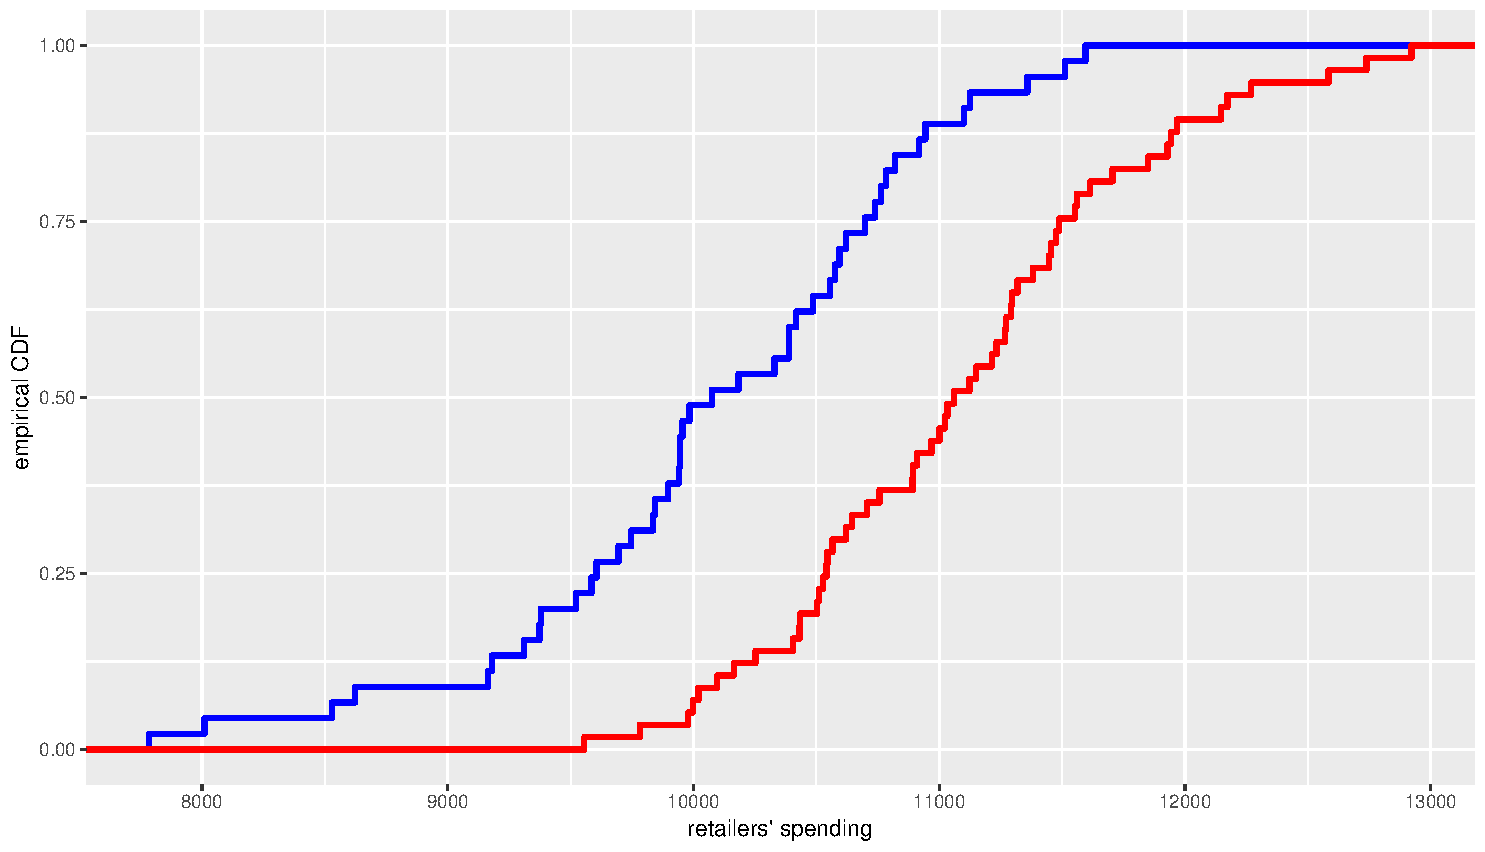
\includegraphics[width=0.99\linewidth]{ecdfs.pdf}
\end{figure}


\begin{enumerate}[(a)]



\subquestionwithpoints{3} Estimate the value of ~$\displaystyle \doublehat{d} := \sup_{x \in \reals} \braces{\abss{\hat{F}_1(x) - \hat{F}_2(x)}}$ as best as possible.

\iftoggle{solutions}{\inred{
At $x \approx 10000$ the difference appears to be maximal at $\doublehat{d} \approx$ \fbox{0.4}.
}}{~\spc{1}}

\subquestionwithpoints{5} At $\alpha=5\%$, make a decision on the suitability of $H_0$, i.e. that spending in the two regions are realized from the same DGP. Note that $F_K(1.36) = 95\%$ where $F_K$ denotes the CDF of Kolmogorov's distribution.

\iftoggle{solutions}{\inred{
 The test statistic for the 2-sample Kolmogorov-Smirnov test is:

\beqn
\doublehat{k} := \sqrt{\frac{n_1 n_2}{n_1 + n_2}} \doublehat{d} = \sqrt{\frac{45 \cdot 57}{45 + 57}} 0.4 = 2.01
\eeqn

where the distance statistic $\doublehat{d}$ was estimated from the plot in the previous question. Since this statistic is larger than the threshold of 1.36 which is given above, we \fbox{reject $H_0$}.
}}{~\spc{5}}

\subquestionwithpoints{1} The test in the previous question is... circle one...\\ exact \quad / \quad \iftoggle{solutions}{\inred{approximate.}}{approximate.}\pagebreak

\end{enumerate}



\problem Consider the following DGP:

\beqn
\Xoneton \iid \text{Laplace}(0, \theta) := \oneover{2\theta} e^{-|x| /\theta}
\eeqn

\noindent Here are some facts about this DGP:

\beqn
\expe{X} = 0,\quad \var{X} = 2\theta^2,\quad \expe{|X|} = \theta
\eeqn

\noindent And below is some of the busy work of the problem done for you:

\beqn
\mathcal{L}(\theta; \X) &=& \prod_{i=1}^n \oneover{2\theta} e^{-|X_i| /\theta} = \oneover{2^n} \oneover{\theta^n} e^{-\displaystyle\oneover{\theta} \displaystyle\sum_{i=1}^n |X_i|} \\
\ell(\theta; \X) &=& -n \natlog{2} -n \natlog{\theta} - \oneover{\theta} \sum_{i=1}^n |X_i| \\
s(\theta; \X) = \ell'(\theta; \X) &=& -\frac{n}{\theta} + \oneover{\theta^2} \sum_{i=1}^n |X_i| \\
0 &=& -\frac{n}{\theta} + \oneover{\theta^2} \sum_{i=1}^n |X_i| \mathimplies n = \oneover{\theta} \sum_{i=1}^n |X_i| \mathimplies \thetahatmle = \oneover{n} \sum_{i=1}^n |X_i| \\
\ell''(\theta; \X) &=& \frac{n}{\theta^2} - 2 \oneover{\theta^3} \sum_{i=1}^n |X_i| \\
\expe{-\ell''(\theta; \X)} &=& \expe{-\frac{n}{\theta^2} + 2 \oneover{\theta^3} \sum_{i=1}^n |X_i|} = 2 \oneover{\theta^3} \expe{\sum_{i=1}^n |X_i|} -\frac{n}{\theta^2} = n \parens{\frac{2\theta}{\theta^3} - \frac{1}{\theta^2}} = \frac{n}{\theta^2}
\eeqn


\begin{enumerate}[(a)]

\subquestionwithpoints{4} What is the asymptotic distribution of $\thetahatmle$? Your answer can only include brand name variable notation, $\theta$, $n$ and fundamental constants. Merely writing the relevant result of the monster theorem will give you one point at most.

\iftoggle{solutions}{\inred{
The relevant result of the monster theorem is:

\beqn
\thetahatmle \approxdist \normnot{\theta}{\frac{I(\theta)^{-1}}{n}} = \normnot{\theta}{\oneover{I_n(\theta)}}
\eeqn

We are given $I_n(\theta)$ in the last line from the problem statement. So we merely substitute:

\beqn
\thetahatmle \approxdist \normnot{\theta}{\frac{\theta^2}{n}} = \normnot{\theta}{\squared{\frac{\theta}{\sqrt{n}}}}
\eeqn\pagebreak
}}{~\spc{7}}


For the rest of this problem, consider the following dataset:

\beqn
\x \,=\, <2.37, 3.71, 0.46, -0.44, 1.37, 9.09, -3.86, -1.69, -3.00, 0.46>
\eeqn

\subquestionwithpoints{6} Compute the maximum likelihood estimate of $\theta$ to the nearest three decimal values.

\iftoggle{solutions}{\inred{
The formula for $\thetahathatmle$ was found for us in the problem statement. Using our calculator:

\beqn
\thetahathatmle &=& \oneover{n} \sum_{i=1}^n |x_i| = \frac{2.37 + 3.71 + 0.46 + 0.44 + 1.37 + 9.09 + 3.86 + 1.69 + 3 + 0.46}{10} \\
&=& \frac{26.45}{10} = 2.645
\eeqn
}}{~\spc{2}}

If you did not answer the previous question, for the rest of the problem, use $\thetahathatmle = 2.645$.

\subquestionwithpoints{6} Calculate a 95\% confidence interval for $\theta$ to the nearest three decimals.

\iftoggle{solutions}{\inred{

\beqn
CI_{\theta, 95\%} &=& \bracks{\thetahathatmle \pm 1.96 \oneoversqrt{I_n\parens{\thetahathatmle}}} \\
&=& \bracks{\thetahathatmle \pm 1.96 \frac{\thetahathatmle}{\sqrt{n}}} = \bracks{2.645 \pm 1.96 \frac{2.645}{\sqrt{10}}} = \bracks{1.006, 4.284}
\eeqn
}}{~\spc{6}}


\subquestionwithpoints{6} Test $H_0: \theta = 2$ using the Wald Test at $\alpha = 5\%$. Your answer must include computing the proper retainment region.

\iftoggle{solutions}{\inred{
The Wald test is the asymptotically valid Z test using the asymptotic normality of $\thetahatmle$. Thus we can compute a retention region:

\beqn
RET_{5\%} &=& \bracks{\theta_0 \pm 1.96 \oneoversqrt{I_n\parens{\theta_0}}} = \bracks{\theta_0 \pm 1.96 \frac{\theta_0}{\sqrt{n}}} = \bracks{2 \pm 1.96 \frac{2}{\sqrt{10}}} = \bracks{0.76, 3.24}
\eeqn

Since $\thetahathatmle = 2.645 \in RET_{5\%}$, we \fbox{fail to reject $H_0$}.
}}{~\spc{6}}
\pagebreak

\subquestionwithpoints{6} Test $H_0: \theta = 2$ using the Score Test at $\alpha = 5\%$. Your answer must include computing the proper test statistic and comparing it to the proper retainment region.

\iftoggle{solutions}{\inred{
The Score test provides an asymptotically valid z test statistic:

\beqn
\doublehat{z} &=& \frac{s(\theta_0; \X)}{\sqrt{I_n(\theta_0)}} = \frac{-\frac{n}{\theta_0} + \oneover{\theta_0^2} \sum_{i=1}^n |x_i|}{\sqrt{\frac{n}{\theta_0^2}}} = \frac{-\frac{10}{2} + \oneover{2^2} 26.45}{\sqrt{\frac{10}{2^2}}} = 1.0198
\eeqn

Since $\doublehat{z} = 1.02 \in RET_{5\%} = \bracks{\pm 1.96}$, we \fbox{fail to reject $H_0$}.
}}{~\spc{7}}

\subquestionwithpoints{6} Test $H_0: \theta = 2$ using the Likelihood Ratio Test at $\alpha = 5\%$. Your answer must include computing the proper test statistic and comparing it to the proper retainment region.

\iftoggle{solutions}{\inred{
The Score test provides an asymptotically valid chi-squared 1 test statistic:

\beqn
\doublehat{\Lambda} &=& 2\parens{\ell(\thetahathatmle; \x) -\ell(\theta_0; \x)} \\
&=& 2\parens{\parens{\cancel{-n \natlog{2}} -n \natlog{\theta} - \oneover{\theta} \sum_{i=1}^n |X_i|} - \parens{\cancel{-n \natlog{2}} -n \natlog{\theta} - \oneover{\theta} \sum_{i=1}^n |X_i|}} \\
&=& 2\parens{\parens{ -n \natlog{\thetahathatmle} - \oneover{\thetahathatmle} \sum_{i=1}^n |X_i|} - \parens{ -n \natlog{\theta_0} - \oneover{\theta_0} \sum_{i=1}^n |X_i|}} \\
&=& 2\parens{ -10 \natlog{2.645} - \oneover{2.645} 26.45 + 10 \natlog{2}  + \oneover{2} 26.45} = 0.8595\\
\eeqn

By the equivalence of z-tests and chi-squared-1 tests, we know that the $RET_{5\%} = \bracks{0, 1.96^2} = \bracks{0, 3.84}$. Since $\doublehat{\Lambda} = 0.8595 \in RET_{5\%}$, we \fbox{fail to reject $H_0$}.
}}{~\spc{7}}


\subquestionwithpoints{4} \\
The interval in (c) is... circle one... exact \quad / \quad \iftoggle{solutions}{\inred{approximate.}}{approximate.} \\
The decision in (d) is... circle one... exact \quad / \quad \iftoggle{solutions}{\inred{approximate.}}{approximate.} \\
The decision in (e) is... circle one... exact \quad / \quad \iftoggle{solutions}{\inred{approximate.}}{approximate.} \\
The decision in (f) is... circle one... exact \quad / \quad \iftoggle{solutions}{\inred{approximate.}}{approximate.}
\pagebreak
\end{enumerate}



\problem Let's consider a scenario where we want to investigate whether there is an association between gender and preference for car models Honda vs Toyota among middle-aged suburbanites in Long Island. We collect the data in a contingency table, where the rows represent gender (Male vs Female), and the columns represent product preference (Honda vs Toyota). We ask an SRS of middle-aged suburbanites in Long Island which model they prefer and their gender. The contingency table of the data is below:

\begin{table}[htp]
    \centering
    \begin{tabular}{c|cc}
 & Honda & Toyota \\
\hline
Male & 17 & 53 \\
Female & 28 & 46 \\
    \end{tabular}
\end{table}

\begin{enumerate}[(a)]

%Let $\theta_M$ be the probability of male, $\theta_F$ be the probability of female, $\theta_H$ be the probability of Honda preference, $\theta_T$ be the probability of Toyota preference, $\theta_{MH}$ be the probability of male and Honda preference,  $\theta_{MT}$ be the probability of male and Toyota preference, $\theta_{FH}$ be the probability of female and Honda preference and $\theta_{FT}$ be the probability of female and Honda preference,

% \subquestionwithpoints{6} What is $n$?

% \iftoggle{solutions}{\inred{
% 144
% }}{~\spc{1}}


\subquestionwithpoints{10} At $\alpha = 5\%$, test the null hypothesis that gender and car model are independent. Your answer must include computing the proper test statistic and comparing it to the proper retainment region.

\iftoggle{solutions}{\inred{
This is a chi-squared test. We first complete the table with empirical probabilities of being in each row and column:

\begin{table}[htp]
    \centering
    \color{red}
    \begin{tabular}{c|cc|c}
 & Honda & Toyota & Total (prob estimate)\\
\hline
Male & 17 & 53 & 70 (.486)\\
Female & 28 & 46 & 74 (.514)\\ \hline
 Total (prob estimate) & 45 (.313) & 99 (.687) & 144
    \end{tabular}
\end{table}

This then allows us to construct expected values under the null of independent via multiplying the row-column probability estimates:


\begin{table}[htp]
    \centering
    \color{red}
    \begin{tabular}{c|cc}
 & Honda & Toyota \\
\hline
Male & 21.875 & 48.125\\
Female & 23.125 & 50.875\\
    \end{tabular}
\end{table}

We now compute Pearson's test statistic:

\beqn
\doublehat{\phi} = \frac{\squared{17-21.875}}{21.875} + \frac{\squared{53-48.125}}{48.125} + \frac{\squared{28-23.125}}{23.125} + \frac{\squared{46-50.875}}{50.875} = 3.075
\eeqn

As there are two rows and two columns, the degrees of freedom on the chi-squared is 1. By the equivalence of z-tests and chi-squared-1 tests, we know that the $RET_{5\%} = \bracks{0, 1.96^2} = \bracks{0, 3.84}$ and thus we \fbox{fail to reject $H_0$}.
}}{~\spc{1}}
\end{enumerate}
\pagebreak

\problem You have measurements of survival of $n = 11$ yeast cultures in a laboratory. Pertinent statistics are $\xbar = 40.3$ and $s = 114.6$. Let $\theta$ denote the mean survival of the yeast cultures.

\begin{enumerate}[(a)]


\subquestionwithpoints{6} Assume the survivals above are iid normally distributed. Compute a $CI_{\theta, 95\%}$ to two decimals. Here are a table of 97.5\%iles of Student's T distribution under a variety of degrees of freedom (df).

\begin{table}[ht]
\centering
\begin{tabular}{r|rrrrrrrrrrrrr}
df & 1 & 2 & 3 & 4 & 5 & 6 & 7 & 8 & 9 & 10 & 11 & 12 & 13 \\ 
   \hline
$F^{-1}(.975)$ & 12.71 & 4.30 & 3.18 & 2.78 & 2.57 & 2.45 & 2.36 & 2.31 & 2.26 & 2.23 & 2.20 & 2.18 & 2.16
\end{tabular}
\end{table}

\iftoggle{solutions}{\inred{

We employ the default estimator for the mean i.e. $\thetahat := \Xbar$ so that

\beqn
CI_{\theta, 95\%} &=& \bracks{\xbar \pm t_{n-1, .975} \frac{s}{\sqrt{n}}} = \bracks{\xbar \pm t_{10, .975} \frac{s}{\sqrt{n}}} = \bracks{40.3 \pm 2.23 \frac{114.6}{\sqrt{11}}} = \bracks{-36.75, 117.35}
\eeqn
}}{~\spc{4}}

\subquestionwithpoints{1} The interval above is... circle one... \iftoggle{solutions}{\inred{exact}}{exact} \quad / \quad approximate.

\subquestionwithpoints{3} What is conceptually wrong with the above CI?

\iftoggle{solutions}{\inred{
It contains negative values. Survival must be positive.
}}{~\spc{2}}


\subquestionwithpoints{8} Let $\phi = \natlog{\theta}$. Compute a $CI_{\phi, 95\%}$ to two decimals.

\iftoggle{solutions}{\inred{
We need to use delta method and the three theorems:

\beqn
\frac{\hat{\phi} - \phi}{|g'(\hat{\theta})| \hat{SE}\bracks{\hat{\theta}}} \convd \stdnormnot 
\eeqn

And when using the finite approximation:

\beqn
CI_{\phi, 95\%} &\approx& \bracks{\doublehat{\phi} \pm 1.96 |g'(\doublehat{\theta})| \doublehat{SE}\bracks{\hat{\theta}}} 
\eeqn

Here, $\doublehat{\theta} = \xbar$ and $\doublehat{SE}\bracks{\hat{\theta}} = \doublehat{SE}\bracks{\Xbar} = \frac{s}{\sqrt{n}}$. Substituting,

\beqn
CI_{\phi, 95\%} &\approx& \bracks{\natlog{\xbar} \pm 1.96 \oneover{\abss{\xbar}} \frac{s}{\sqrt{n}}} = \bracks{\natlog{40.3} \pm 1.96 \frac{114.6}{40.3\sqrt{11}}} = \bracks{2.02, 5.38}
\eeqn

}}{~\spc{1}}

\end{enumerate}
\pagebreak

\problem Consider $\Xoneton \iid \bernoulli{\theta}$ and the Laplace principle of indifference prior on the entire parameter space, $\Theta = (0,1)$.

\begin{enumerate}[(a)]


\subquestionwithpoints{8}  Find the posterior distribution step-by-step from first principles. If it's a brand-name rv, mark it so and provide the values of its parameters.

\iftoggle{solutions}{\inred{

\beqn
f(\theta~|~\X) &=& \frac{\cprob{\X}{\theta} f(\theta)}{\prob{\X}} \propto \cprob{\X}{\theta} f(\theta) \\
&=& \parens{\prod_{i=1}^n \theta^{x_i} (1-\theta)^{1-x_i}} \indic{\theta \in (0,1)} \\
&=& \theta^{\sum x_i} (1-\theta)^{\sum 1-x_i} \indic{\theta \in (0,1)} \\
&=& \theta^{\sum x_i +1 - 1} (1-\theta)^{n-\sum x_i + 1 -1} \indic{\theta \in (0,1)} \\
&\propto& \betanot{1 + \sum_{i=1}^n x_i}{1 + n - \sum_{i=1}^n x_i}
\eeqn

}}{~\spc{1}}

\end{enumerate}

\end{document}

















\problem Let $X_1, X_2, \ldots \iid$ some continuous random variable with $0 < \mu < \infty$ and $0 < \sigsq < \infty$. We also use the standard notation 

\beqn
\Xbar_n := \oneover{n}\sum_{i=1}^n X_i ~~~~\text{and}~~~~ S^2_n := \oneover{n-1} \sum_{i=1}^n (X_i - \Xbar_n)^2.
\eeqn

\begin{enumerate}[(a)]



\subquestionwithpoints{6} Use Chebyshev's inequality to prove the WLLN, i.e., that $\Xbar_n \convp \mu$.

\iftoggle{solutions}{\inred{
\beqn
\forall \epsilon > 0, ~~\limitn \prob{|\Xbar_n - \mu| \geq \epsilon} \leq \limitn \frac{\var{\Xbar_n}}{\epsilon} = \limitn \frac{\sigsq / n}{\epsilon} = 0 ~~\checkmark
\eeqn
}}{~\spc{8}}


\subquestionwithpoints{6} Assume $n$ is large. Plot the approximate PDF of $\Xbar_n$ denoted $f_{\Xbar_n}(\xbar)$. Label the horizontal and vertical axes. Indicate critical value(s) on the axes.

\iftoggle{solutions}{\inred{

By the WLLN, $\Xbar_n \convp \mu$, which means that as $n$ gets larger, all the probability \qu{piles up} near $\mu$ and since we assumed $\mu > 0$, we should get something like this:

\begin{figure}[htp]
    \centering
    \includegraphics[width=0.75\linewidth]{Xbar_approx_PDF_plot.jpg}
\end{figure}\pagebreak
}}{~\spc{7}}

\subquestionwithpoints{8}  Using the fact that $S^2_n \convp \sigsq$ and the theorems we learned about in class, show the following fact about the ratio Student was investigating at the turn of the century:

\beqn
\frac{\Xbar_n - \mu}{\frac{S}{\sqrt{n}}} ~\convd~ \stdnormnot
\eeqn

\iftoggle{solutions}{\inred{
Using the fact given above, $S \convp \sigma$ by the CMT where $g(t) = \sqrt{t}$. Then, $\frac{\sigma}{S} \convp 1$ by the CMT where $g(t) = t/\sigma$.
\beqn
\frac{\Xbar_n - \mu}{\frac{S}{\sqrt{n}}} = \overbrace{\underbrace{\frac{\sigma}{S}}_{\text{see above}}\underbrace{\frac{\Xbar_n - \mu}{\frac{\sigma}{\sqrt{n}}}}_{\convd \stdnormnot ~~\text{by CLT}} ~\convd~ \stdnormnot}^{\text{by Slutsky's A theorem}}
\eeqn
}}{~\spc{6}}


% \subquestionwithpoints{3} How is the following rv approximately distributed? Provide theoretical justification for each step.

% \beqn
% \frac{n+1}{n+2} + \frac{\sqrt{n}\Xbar_n - \sqrt{n}\mu}{\sigma} \hspace{20cm} 
% \eeqn

% \iftoggle{solutions}{\inred{
% $\braces{1,2,\ldots,9}$
% }}{~\spc{5}}

For the remainder of the questions in this problem, assume that

\beqn
\Xoneton \iid \normnot{\mu}{\sigsq}
\eeqn

\subquestionwithpoints{3} Let $Z_i := (X_i - \mu) / \sigma$. How are following distributed?

\beqn
Z_1, \ldots, Z_n \iftoggle{solutions}{\inred{\iid \stdnormnot}}{\hspace{20cm}}
\eeqn


\subquestionwithpoints{4} The following has a brand name distribution. Find this distribution and its parameter(s).

\iftoggle{solutions}{\inred{The ratio of two independent standard normals was proved in class to be a Cauchy(0,1). Below is just a linear transformation yielding}}

\beqn
17 + 37\frac{Z_7}{Z_{11}} \iftoggle{solutions}{\inred{\sim \cauchynot{17}{37}}}{\hspace{20cm}\spc{4}}
\eeqn

\subquestionwithpoints{4} The following has a brand name distribution. Find this distribution and its parameter(s).

\iftoggle{solutions}{\inred{
\beqn
\frac{{\displaystyle\frac{\Xbar_n - \mu}{\frac{\sigma}{\sqrt{n}}}}}{\sqrt{\frac{\frac{n-1}{\sigsq} S^2_n}{n-1}} } = \frac{\Xbar_n - \mu}{\frac{S_n}{\sqrt{n}}} \sim T_{n-1}
\eeqn

Where the equality follows from algebraic simplification.
\pagebreak
}}{
\beqn
\frac{{\displaystyle\frac{\Xbar_n - \mu}{\frac{\sigma}{\sqrt{n}}}}}{\sqrt{\frac{\frac{n-1}{\sigsq} S^2_n}{n-1}} } \hspace{20cm}
\eeqn
~\spc{0}
}

\subquestionwithpoints{7} The following has a brand name distribution. Find this distribution and its parameter(s).

\iftoggle{solutions}{\inred{
\beqn
\frac{\frac{n-1}{\sigsq} S^2_n}{\squared{\displaystyle\frac{\Xbar_n - \mu}{\frac{\sigma}{\sqrt{n}}}}}=: R = \frac{U}{V^2}
\eeqn
}}{
\beqn
\frac{\frac{n-1}{\sigsq} S^2_n}{\squared{\displaystyle\frac{\Xbar_n - \mu}{\frac{\sigma}{\sqrt{n}}}}} \hspace{20cm}
\eeqn
~\spc{7}
}

\iftoggle{solutions}{\inred{
We know from class that $U \sim \chisq{n-1} = \gammanot{\frac{n-1}{2}}{\half}$ and $V \sim \stdnormnot$ which imples $V^2 \sim \chisq{1}  =\gammanot{\half}{\half}$. By Cochran's theorem, $U$ and $V$ are independent. Thus, $R$ is a ratio of two independent gamma rv's that share their $\beta$ parameter value. We proved in class that such a ratio is beta prime with first parameter given by the first parameter of the numerator and second parameter given by the first parameter of the denominator,

\beqn
R \sim \text{BetaPrime}\parens{\frac{n-1}{2}, \half}
\eeqn
}}

\subquestionwithpoints{7} The following expression is distributed as a brand name variable. Find the brand name variable and its parameter values:

\iftoggle{solutions}{
\inred{
\beqn
n\Xbar_n^2 - 2n\mu\Xbar_n + n\mu^2 + nS^2_n - S^2_n &=& n\squared{\Xbar_n - \mu} + (n-1)S^2_n} \\
&=& \frac{\sigsq}{\sigsq}\parens{n\squared{\Xbar_n - \mu} + (n-1)S^2_n} \\
&=& \sigsq \parens{\squared{\frac{\Xbar_n - \mu}{\frac{\sigma}{\sqrt{n}}}} + \frac{n-1}{\sigsq}S^2_n} \\
&\sim& \gammanot{\frac{n}{2}}{\oneover{2\sigsq}}
\eeqn

Let's examine the term inside the parentheses on the third line. By Cochran's theorem, the first term is $\chisq{1}$ and the second term is $\chisq{n-1}$ and both terms are independent. Thus the entire parenthesis is distributed as $\chisq{n} = \gammanot{\frac{n}{2}}{\half}$. Hence we are scaling a gamma by $\sigsq$ which yields another gamma distribution with its $\beta$ parameter divided by the scaling value. \pagebreak
}{
\beqn
n\Xbar_n^2 - 2n\mu\Xbar_n + n\mu^2 + nS^2_n - S^2_n\hspace{20cm}
\eeqn
~\spc{7}}





\end{enumerate}


\problem Some theoretical problems. 

\begin{enumerate}[(a)]


\subquestionwithpoints{7} Let $X \sim \text{Weibull}(k, \lambda)$. Find the most succinct expression as possible for $\expe{X}$. I have started you off below. Hint: the solution contains a gamma function.

\beqn
\expe{X} = \int_\reals x f_X(x) dx = \int_\reals x \parens{k\lambda (\lambda x)^{k-1} e^{-(\lambda x)^k}} \indic{x>0}~ dx = k\lambda^k \int_0^\infty x^k e^{-\lambda^k x^k} dx
\eeqn

\iftoggle{solutions}{\inred{
Let $u = x^k$ thus $x = u^{1/k}$, $du/dx = k x^{k-1}$, $dx = 1/(kx^{k-1})du$ and the bounds of the integration do not change. Using this substitution,

\beqn
\expe{X} = k\lambda^k \int_0^\infty x^k e^{-\lambda^k u} 1/(kx^{k-1})du = \lambda^k \int_0^\infty x e^{-\lambda^k u} du = \lambda^k \int_0^\infty u^{1/k} e^{-\lambda^k u} du
\eeqn

Since $u^{1/k} = u^{1/k +1 - 1}$, we have a gamma-like integral with $\alpha = 1/k + 1$ and $c = \lambda^k$:

\beqn
\expe{X} = \lambda^k \int_0^\infty u^{\alpha - 1} e^{-c u} du = \lambda^k \frac{\Gamma(\alpha)}{c^\alpha} = \lambda^k \frac{\Gamma(1/k + 1)}{\tothepow{\lambda^k}{1/k + 1}} = \lambda^k \frac{\Gamma(1/k + 1)}{\lambda^{1 + k}} = \oneover{\lambda} \Gamma(1/k + 1)
\eeqn
}}{~\spc{7}}


\subquestionwithpoints{7} Let $X \sim \text{ParetoI}(k, \lambda)$. Find the distribution of $Y = X ~|~X>c$ where $c>k$. If it's a brand-name rv, mark it as its brand name and find its parameters.

\iftoggle{solutions}{\inred{
The trick here is to use the survival function of the ParetoI, $S_X(x) := 1 - F_X(x) = \tothepow{\frac{k}{x}}{\lambda}$
\beqn
S_Y(y) &:=& \prob{Y > y} = \cprob{X > y}{X > c} = \frac{\prob{X > y, X > c}}{\prob{X > c}} = \frac{\prob{X > y}}{\prob{X > c}} \\
&=& \frac{S_X(y)}{S_X(c)} = \frac{\tothepow{\frac{k}{y}}{\lambda}}{\tothepow{\frac{k}{c}}{\lambda}} = \tothepow{\frac{c}{y}}{\lambda} \mathimplies Y \sim \text{ParetoI}(c, \lambda)
\eeqn

Survival functions characterize a distribution (just like CDF's, PDF's, PMF's, chf's).
\pagebreak
}}{~\spc{8}}

\subquestionwithpoints{3} Let $\X \sim \text{Mult}_3\parens{9, \oneover{3} \onevec_3}$. Find the distribution of $Y = \onevec_k^\top \X$ where $k$ is the appropriate dimension to make the vector operation legal.

\iftoggle{solutions}{\inred{
\beqn
Y = \onevec_3^\top \X = X_1 + X_2 + X_3 \sim \text{Deg}(9)
\eeqn
}}{~\spc{3}}

\subquestionwithpoints{5} Let $\X \sim \text{Mult}_3\parens{9, \oneover{3} \onevec_3}$. Find $\var{\X}$. Simplify your answer so that it is a function of $\I_3$, the identity matrix and $\bv{J}_3$, the matrix of all ones.

\iftoggle{solutions}{\inred{
Note: $\bv{p} = \oneover{3} \onevec_3$ which means $p_1 = p_2 = p_3 = \oneover{3}$ thus we just plug in these values to the formula from class and simplify:

\beqn
\var{\X} = n\bracks{\begin{array}{ccc} 
p_1 (1-p_1) & -p_1 p_2 & -p_1 p_3 \\
-p_2 p_1 & p_2 (1-p_2) & -p_2 p_3 \\
-p_3 p_1 & -p_3 p_2 & p_3 (1-p_3)
\end{array}} = \frac{9}{9}\bracks{\begin{array}{ccc} 
2 & -1 & -1 \\
-1 & 2 & -1 \\
-1 & -1 & 2
\end{array}} = 3\I_3 - \bv{J}_3
\eeqn
}}{~\spc{6}}

\subquestionwithpoints{7} If $X \sim \text{Laplace}(0,1)$ and $Y = e^X$. Find $f_Y(y)$ in simplest form.

\iftoggle{solutions}{\inred{
\beqn
X &\sim& \text{Laplace}(0,1) := \half e^{-|x|} \indic{x \in \reals}, \quad X = \natlog{Y} = g^{-1}(Y) \mathimplies \frac{d}{dy}\bracks{g^{-1}(y)} = \oneover{y} \\
f_Y(y) &=& f_X(g^{-1}(y))\abss{\frac{d}{dy}\bracks{g^{-1}(y)}} = \half e^{-|(\natlog{y})|} \indic{\natlog{y} \in \reals} \oneover{|y|} = \oneover{2y} e^{-|\natlog{y}|} \indic{y \in (0, \infty)} \\
&=& \half \begin{cases}
y^{-2} ~~\text{if}~~ y \geq 1 \\
1 ~~\text{if}~~ y \in (0,1) \\
0 ~~\text{if}~~ y \leq 0
\end{cases}
\eeqn

% pacman::p_load(ggplot2)

% Nsim = 1000
% xs = array(NA, Nsim)
% bs = runif(Nsim) > 0.5
% rs = rexp(Nsim)
% for (nsim in 1 : Nsim){
%   xs[Nsim] = exp(bs[Nsim] * rs[Nsim])
% }

% ggplot(data.frame(xs = xs)) + 
%   geom_histogram(aes(x = xs))

(The piecewise function notation is the simplest form but it is not needed for full credit).\pagebreak
}}{~\spc{10}}

\subquestionwithpoints{4} If $X \sim F_{2\alpha, 2\beta}$, find $k_X(x)$ in simplest form.

\iftoggle{solutions}{\inred{
\beqn
f_X(x) &\propto& x^{\overtwo{2\alpha} - 1} \tothepow{1 + \frac{2\alpha}{2\beta}x}{-\overtwo{2\alpha + 2\beta}} \indic{x > 0} = x^{\alpha - 1} \tothepow{1 + \frac{\alpha}{\beta}x}{-(\alpha + \beta)} \indic{x > 0} = k_X(x)\\
\eeqn
}}{~\spc{4}}

\subquestionwithpoints{7} If $X \sim F_{2\alpha, 2\beta}$, find the distribution of $Y = \frac{\alpha}{\beta}X$. If it is a brand-name distribution, indicate which one and the values of its parameter(s). Hint: use kernels.

\iftoggle{solutions}{\inred{
Because the parameter space of the F distribution is two positive parameters, we know $\alpha > 0$ and $\beta > 0$. We make use of $k_X(x)$ from the previous problem

\beqn
f_Y(y) &=& \oneover{\frac{\alpha}{\beta}} f_X\parens{\oneover{\frac{\alpha}{\beta}}y} \propto f_X\parens{\frac{\beta}{\alpha}y} \propto k_X\parens{\frac{\beta}{\alpha}y} =  \tothepow{\frac{\beta}{\alpha}y}{\alpha - 1} \tothepow{1 + \frac{\alpha}{\beta}\parens{\frac{\beta}{\alpha}y}}{-(\alpha + \beta)} \indic{\parens{\frac{\beta}{\alpha}y} > 0} \\
&\propto& y^{\alpha - 1} \tothepow{1 + y}{-(\alpha + \beta)} \indic{y > 0} = \frac{y^{\alpha - 1}}{\tothepow{1 + y}{\alpha + \beta}} \indic{y > 0} \propto \text{BetaPrime}(\alpha,\beta)
\eeqn
}}{~\spc{8}}


\subquestionwithpoints{5} If $X \sim \bernoulli{p} := p^x (1-p)^{1-x} \indic{x \,\in\, \braces{0,1}}$, find the PMF of $Y = e^X$ in simplest form. Your answer should contain a $\indic{y \,\in\, \support{Y}}$ term where $\support{Y}$ is an explicit set.

\iftoggle{solutions}{\inred{
\beqn
X &=& \natlog{Y} = g^{-1}(Y) \\
p_Y(y) &=& p_X(g^{-1}(y)) \\
&=& p^{\natlog{y}} (1-p)^{1-\natlog{y}} \indic{\natlog{y} \,\in\, \braces{0,1}} \\
&=& p^{\natlog{y}} (1-p)^{1-\natlog{y}} \indic{y \,\in\, \braces{1,e}}
\eeqn
\pagebreak
}}{~\spc{4}}



\subquestionwithpoints{3} If $X \sim \text{ExtNegBin}(k,p)$ where $k > 0$ and $p \in (0,1)$, what is $\support{X}$? \iftoggle{solutions}{\inred{
$\naturals_0$
}}{~\spc{1.5}}


\subquestionwithpoints{7} Underline all the following distributions which are considered \qu{waiting time distributions}. Then, draw a rectangle box around all the following distributions which are considered \qu{error distributions}.\\

\iftoggle{solutions}{\inred{
\underline{Erlang(4, 0.3)} \quad \underline{Gamma($\pi$, e)} \quad \underline{$\chisq{17}$} \quad $\normnot{1}{2^2}$ \quad \fbox{$T_7$} \quad \underline{$F_{3,6}$} \quad \underline{Weibull(1.6, 0.9)}\\~\\ 
Mult$_3(18, \third \onevec_3$) \quad \underline{BetaPrime(6.1,9.7)} \quad \fbox{Logistic(0,1)} \quad \fbox{Laplace(0, $\pi$)} \\~\\ \underline{LogNormal(1,2)} \quad ParetoI(7,17) \quad Gumbel(0,1)
}}{
Erlang(4, 0.3)\quad Gamma($\pi$, e) \quad $\chisq{17}$ \quad $\normnot{1}{2^2}$ \quad $T_7$ \quad $F_{3,6}$ \quad Weibull(1.6, 0.9)\\~\\~\\
Mult$_3(18, \third \onevec_3$) \quad BetaPrime(6.1,9.7) \quad Logistic(0,1) \quad Laplace(0, $\pi$) \\~\\~\\ 
LogNormal(1,2) \quad ParetoI(7,17) \quad Gumbel(0,1)
}



\end{enumerate}

\end{document}

\problem This problem is about a random phenomenon called Benford's Law, it represents the distribution of leading digit in data across a wide variety of data sets that measure natural phenomenon such as street addresses, stock prices, population numbers, etc. Letting $x$ be the digit in base 10, we have the following rv which has mean and variance:

\beqn
X \sim \text{Benford} := \logbaseten{\frac{x+1}{x}} \indic{x \in \braces{1, 2, \ldots, 9}}, \quad \expe{X} = 3.44, \quad \var{X} = 6.06
\eeqn
%\quad \phi_X(t) = \sum_{x\in \reals} e^{itx} ~\logbaseten{\frac{x+1}{x}} \indic{x \in \braces{1, 2, \ldots, 9}}, 

\begin{enumerate}[(a)]


\subquestionwithpoints{3} What is the support of $X$? $\support{X}$ = \iftoggle{solutions}{\inred{$\braces{1,2,\ldots,9}$}}

\subquestionwithpoints{3} Circle one: this rv is... \quad \iftoggle{solutions}{\inred{discrete}}{discrete} \quad / \quad continuous \quad

\subquestionwithpoints{3} Circle one: the PMF (or PDF) of $X$  is in... \quad old-style \quad / \quad \iftoggle{solutions}{\inred{new style}}{new style}

\subquestionwithpoints{3} Circle one: $X$ ... \quad has parameter(s) \quad / \quad \iftoggle{solutions}{\inred{does not have parameter(s)}}{does not have parameter(s)}\quad

\subquestionwithpoints{6} Find $\prob{X \leq 3}$ exactly and then approximate to the nearest 3 decimals.

\iftoggle{solutions}{\inred{
\beqn
\prob{X=1} + \prob{X=2} + \prob{X=3} = \logbaseten{\frac{2}{1}} + \logbaseten{\frac{3}{2}} + \logbaseten{\frac{4}{3}} = 0.602
\eeqn
}}{~\spc{3}}

\subquestionwithpoints{7} Verify the Humpty-Dumpty Identity for the PMF (or PDF). Hint: remember the precalculus rule that $\text{log$_{10}$}(a/b) = \text{log$_{10}$}(a) - \text{log$_{10}$}(b)$.

\iftoggle{solutions}{\inred{
\beqn
&& \sum_{x \in \braces{1,2, \ldots, 9}}\logbaseten{\frac{x+1}{x}} = \sum_{x \in \braces{1,2, \ldots, 9}}\logbaseten{x+1} - \sum_{x \in \braces{1,2, \ldots, 9}} \logbaseten{x} \\
&=& \sum_{x \in \braces{2,3, \ldots, 10}}\logbaseten{x} - \sum_{x \in \braces{1,2, \ldots, 9}} \logbaseten{x} = \cancelto{1}{\logbaseten{10}} - \cancelto{0}{\logbaseten{1}} = 1 ~\checkmark
\eeqn
}}{~\spc{5}}

\subquestionwithpoints{7} Find an expression for $F_X(x)$, the CDF of $X$, that is valid for all $x \in \reals$.  Hint: one possible answer has $|\support{X}|$ terms and each includes an indicator function.


\iftoggle{solutions}{\inred{
\beqn
F_X(x) &=& \logbaseten{\frac{2}{1}} \indic{x \geq 1} + \logbaseten{\frac{3}{2}} \indic{x \geq 2} + \ldots + \logbaseten{\frac{10}{9}} \indic{x \geq 9}  \\
&=& \sum_{i \in \braces{1,2, \ldots, 9}} \logbaseten{\frac{i+1}{i}} \indic{x \geq i}
\eeqn
\pagebreak
}}{~\spc{3}}

% \subquestionwithpoints{4} Using the chf of $X$, find an expression that computes $\expe{X}$.\spc{3}

\subquestionwithpoints{10} Find an upper bound for $\expe{X^4}$ to the nearest two decimals. Hint: use the Cauchy-Schwartz inequality.


\iftoggle{solutions}{\inred{
\beqn
\expe{X^4} = \abss{\expe{X^4}} = \abss{\expe{X X^3}}  &\leq& \sqrt{\expe{X^2} \expe{X^6}} = \abss{\expe{X^2}} = \expe{X^2} = \var{X} + \expe{X}^2 \\
&=& 6.06 + 3.44^2 = 17.89
\eeqn
}}{~\spc{5}}


\subquestionwithpoints{10} Let $Y_n := \oneover{n} X$. Show $Y_n \convd 0$. Hint: $\phi_X(t) = \displaystyle\sum_{x \in \braces{1, 2, \ldots, 9}} e^{itx} \logbaseten{\frac{x+1}{x}}$.

\iftoggle{solutions}{\inred{
\beqn
\limitn \phi_{Y_n}(t) &=& \limitn \phi_{X_n}(t/n) = \limitn \sum_{x \in \braces{1, 2, \ldots, 9}} e^{i\frac{t}{n}x} \logbaseten{\frac{x+1}{x}} \\
&=& \sum_{x \in \braces{1, 2, \ldots, 9}}  \logbaseten{\frac{x+1}{x}} e^{ix \limitn \frac{t}{n}} = \sum_{x \in \braces{1, 2, \ldots, 9}}  \logbaseten{\frac{x+1}{x}} e^{ix (0)} \\
&=& \sum_{x \in \braces{1, 2, \ldots, 9}}  \logbaseten{\frac{x+1}{x}} = 1 = e^{it(0)} = \phi_Y(t) \mathimplies Y_n \convd Y \sim \text{Deg(0)} = 0~\checkmark
\eeqn
}}{~\spc{5}}




% \subquestionwithpoints{4} Find the PMF (or PDF) of $T_2$ valid for all $t \in \reals$. Simplify as much as possible.\spc{6}


\subquestionwithpoints{10} Benford's Law is used by the Internal Revenue Service (IRS) to catch people committing tax fraud. The \qu{1040 form} the IRS uses has about 100 numeric entries. When people commit fraud, they may fabricate numbers by drawing iid from $U(\braces{1,2, \ldots, 9})$ which has mean 5 and thus an average probability of first digit greater than 5 of 4/9. 

If the 100 first digits on the IRS form were distributed according to Benford's Law, what is the approximate probability the average value of the first digit on the IRS 1040 form is greater than 5?


\iftoggle{solutions}{\inred{
\beqn
\Xbar_{100} &\approxdist& \normnot{\expe{X}}{\frac{\var{X}}{100}} = \normnot{3.44}{\frac{6.06}{100}} ~~~\text{by the CLT} \\
\prob{\Xbar_{100} > 5} &\approx& \prob{Z > \frac{5 - 3.44}{\sqrt{\frac{6.06}{100}}}} = \prob{Z > 6.34} \approx 0
\eeqn
\pagebreak
}}{~\spc{6}}


\beqn
\text{Consider} ~~ X_1, X_2 \iid \text{Benford} \quad \text{and} \quad T_2 := X_1 + X_2  \hspace{6cm}
\eeqn


% \subquestionwithpoints{3} What real value is the following expression close to?

% \beqn
% \frac{X_1 + X_2 + \ldots + X_{100}}{100} \approx \hspace{11cm}
% \eeqn

% \subquestionwithpoints{3} Let $t_n$ be a realization from the rv $T_n$. What is the best approximation for the value of $t_{100}$? Your answer must be a real number.\spc{2}

\subquestionwithpoints{3} Find the covariance, $\cov{X_1}{X_2} =$ \iftoggle{solutions}{\inred{0 (due to independence)}}


\subquestionwithpoints{3} What is the support of $T_2$? $\support{T_2}$ = \iftoggle{solutions}{\inred{$\braces{2,3, \ldots, 18}$}}

\end{enumerate}

\problem 
\beqn
\text{Consider the following rv:}~~X, Y \iid \frac{\lambda-1}{(x+1)^{\lambda}} \indic{x \in (0, \infty)}, \quad T = X+Y
\eeqn

\begin{enumerate}[(a)]
\subquestionwithpoints{3} What is the support of $X$? $\support{X}$ = \iftoggle{solutions}{\inred{$(0, \infty)$}}

\subquestionwithpoints{3} Circle one: this rv is... \quad discrete \quad / \quad \iftoggle{solutions}{\inred{continuous}}{continuous} \quad

\subquestionwithpoints{3} Circle one: the PMF (or PDF) of $X$  is in... \quad old-style \quad / \quad \iftoggle{solutions}{\inred{new style}}{new style}

\subquestionwithpoints{3} Circle one: $X$ ... \quad \iftoggle{solutions}{\inred{has parameter(s)}}{has parameter(s)} \quad / \quad does not have parameter(s)\quad


\subquestionwithpoints{10} Find the PMF (or PDF) of $T$ valid for all $ t\in\reals$. Leave in sum (or definite integral) format but factor out all constants and simplify \emph{as much as possible}.


\iftoggle{solutions}{\inred{
\beqn
f_T(t) &=& \int_{\support{X}} f(x) f(t-x) \indic{t-x \in \support{X}} ~dx = \int_{x \in (0, \infty)} \frac{\lambda-1}{(x+1)^{\lambda}} \frac{\lambda-1}{(t-x+1)^{\lambda}} \indic{t-x \in (0, \infty)} ~dx \\
&=& (\lambda - 1)^2 \int_{x \in (0, \infty)} \oneover{((x+1)(t-x+1))^\lambda} \indic{x \in (-\infty, t)} ~dx \\
&=& (\lambda - 1)^2 \indic{t \in (0, \infty)} \int_{x \in (0, t)} \oneover{((x+1)(t-x+1))^\lambda} ~dx
\eeqn
}}{~\spc{5}}

\subquestionwithpoints{10} Find $\prob{X > Y}$. Leave in sum (or definite integral) format but factor out all constants and simplify \emph{as much as possible}.


\iftoggle{solutions}{\inred{
\beqn
\prob{X > Y} &=& \int_{y \in \reals} \int_{x \in \reals} f_{X,Y}(x,y) \indic{x > y}~dx dy \\
&=& \int_{y \in \reals} \int_{x \in \reals} \frac{\lambda-1}{(x+1)^{\lambda}} \indic{x \in (0, \infty)} \frac{\lambda-1}{(y+1)^{\lambda}} \indic{y \in (0, \infty)} \indic{x \in (y, \infty)}~dx dy \\
&=&  (\lambda - 1)^2 \int_{y \in (0, \infty)} \frac{1}{(y+1)^{\lambda}} 
 \int_{x \in (0, \infty)} \frac{1}{(x+1)^{\lambda}} \indic{x \in (y, \infty)}~dx dy \\
&=&  (\lambda - 1)^2 \int_{y \in (0, \infty)} \frac{1}{(y+1)^{\lambda}} 
 \int_{x \in (y, \infty)} \frac{1}{(x+1)^{\lambda}} ~dx dy \\
\eeqn
}}{~\spc{5}}

\end{enumerate}
\end{document}

\problem This problem is about a new rv,

\beqn
X \sim \poisson{\lambda} := \frac{\lambda^x e^{-\lambda}}{x!} \indic{x \in \naturals_0} 
\eeqn

\noindent whose parameter space for its sole parameter is $\lambda > 0$.


\begin{enumerate}[(a)]


\subquestionwithpoints{3} What is the support of $X$? $\support{X}$ = 

\subquestionwithpoints{4} Circle one: this rv is \quad discrete \quad / \quad continuous.


\subquestionwithpoints{4} $p^{old}(x) = $\spc{0}


\subquestionwithpoints{5} $\prob{X \in [-2,2]} = $\spc{0}

\subquestionwithpoints{7} Recall the Taylor series for the exponential function of $a$ where $a \in \reals$:

\beqn
e^a = 1 + a + \frac{a^2}{2!} + \frac{a^3}{3!} + \frac{a^4}{4!} + \ldots \quad\quad\quad\quad\quad\quad\quad\quad
\eeqn

Using this fact, prove the Humpty-dumpty rule for the PMF of $X$.\spc{5}

\subquestionwithpoints{6} Write an expression for the CDF of $X$ below denoted $F_X(x)$. For simplicity, assume only $x \in \support{X}$ will be evaluated by this function. Note: the CDF is not available in closed form. Simplify as much as possible. \spc{6}

\subquestionwithpoints{7} Recall the following combinatorial identity from Math 241:

\beqn
\sum_{i=0}^n \binom{n}{i} = 2^n
\eeqn

Let $X_1, X_2 \iid \poisson{\lambda}$ and $T = X_1 + X_2$. Prove the convolution of $p_T(t) = p_{X_1}(x) \star p_{X_2}(x)$ is Poisson and find its parameter value. You may not use characteristic functions to solve this problem. For maximum partial credit, provide the appropriate formula for the convolution and justify each intermediate step. This question is difficult. You may want to do parts (h) and (i) before doing this problem. \spc{9}

\subquestionwithpoints{6} Prove $\phi_X(t) = e^{\lambda (e^{it} - 1)}$. For maximum partial credit, provide the definition of the ch.f. and justify each intermediate step. \spc{10}

\subquestionwithpoints{5} Let $X_1, X_2 \iid \poisson{\lambda}$ and $T = X_1 + X_2$. Using the characteristic function of the Poisson, prove that $T$ is a Poisson rv and find its parameter value. Justify each step. \spc{6}


\subquestionwithpoints{6} Let $X_1, X_2, \ldots, X_n \iid \poisson{17}$ and let $\Xbar_n = \oneover{n}(X_1 + \ldots + X_n)$. If $n$ is very large, what real-number value will $\xbar_n$ be approximately equal to and why? Hint: for $X \sim \poisson{\lambda}$, then $\phi'_X(t)= i\lambda e^{it} e^{\lambda e^{it}} e^{-\lambda}$.\spc{6}

\subquestionwithpoints{6} Let $X_n \sim \poisson{\lambda / n}$, $n \in \naturals$. Prove that $X_n \convd 0$. Justify each step.\spc{6}

\end{enumerate}


\problem Consider rolling a fair die 21 times. The die has 6 sides marked 1, 2, 3, 4, 5, 6 where the side that faces up upon the rolling of the die is uniform discrete.

\begin{enumerate}

\subquestionwithpoints{6} Find an expression for the probability of getting one 1, two 2's, three 3's, four 4's, five 5's and six 6's where the order of those rolls does not matter.\spc{4}

\subquestionwithpoints{6} If $X_1$ is the rv that represents the number of 1's rolled in the 21 rolls, find an expression for $\prob{X_1 = x}$ where $x$ can be any real number.\spc{3}

\end{enumerate}

\problem This problem has disconnected theory questions.

\begin{enumerate}

\subquestionwithpoints{6} Prove that $\cov{aX}{X} = a\var{X}$ from the definition of covariance.\spc{3}

\subquestionwithpoints{6} Let $X$ be a discrete non-negative non-degenerate rv. Prove that $\expe{X} > 0$.\spc{4}

\subquestionwithpoints{5} Under what condition(s) is the following identity true?

\beqn
g(t) = \int_\reals e^{2\pi i\omega t} \int_\reals e^{-2\pi i\omega t} g(t) dt d\omega.
\eeqn\spc{4}


\subquestionwithpoints{6} Let $X_1, \ldots, X_n \iid $ with mean 1 and variance 2. Let $T = X_1 + \ldots + X_n$. Find the approximate probability $T > 3$. Leave your answer in terms of the $\Phi$ function.\spc{4}

\subquestionwithpoints{6}  Let $X \sim \erlang{4}{2}$. Find an integral expression for $\prob{X > 3}$. Simplify as much as possible.

\end{enumerate}

\end{document}





\vspace{-0.2cm}\benum\truefalsesubquestionwithpoints{18} 

\begin{enumerate}[(a)]





\item $\sum_{x \in \reals} \indic{x \in \braces{a}} = a$
\item $\sum_{x \in \reals} \indic{x \in \braces{a}} = 1$
\item $\sum_{x \in \reals} a\indic{x \in \braces{a}} = a$
\item $\sum_{x \in \reals} a\indic{x \in \braces{a}} = 1$
\item $\prod_{x \in \reals} a\indic{x \in \braces{a}} = a$
\item $\prod_{x \in \reals} a\indic{x \in \braces{a}} = 1$  

\item $\int_{\reals} a\indic{x \in [a,b]} = a$  
\item $\int_{\reals} a\indic{x \in [a,b]} = b$  
\item $\int_{\reals} a\indic{x \in [a,b]} = b-a$
\item $\int_0^1 \indic{x \in [a,b]} = b-a$



\item $p(x) = p^{old}(x)\indic{x \in \support{X}}$
\item $\sum_{x \in \reals} p^{old}(x) = 1$
\item $\sum_{x \in \support{X}} p^{old}(x) = 1$

\item $\sum_{x \in \naturals} p(x) = 1$
\item $\sum_{x \in \integers} p(x) = 1$

\item $\int_{\reals} p^{old}(x) = 1$
\item $\int_{\support{X}} p^{old}(x) = 1$

\item $\sum_{x \in \support{X}} p^{old}(x)^2 = 1$

\end{enumerate}
\eenum\instr\pagebreak


%%%%%%%%%%%%%%%%%%
\problem\timedsection{11} Let $X \sim U(\braces{1,2,3})$ and $Y \sim U(\braces{-1,-2,-3})$ and $T = X + Y$.

\vspace{-0.2cm}\benum\truefalsesubquestionwithpoints{19} 

\begin{enumerate}[(a)]
\item $\sum_{x \in \reals} p_{X,Y}(x,y) = 1$
\item $p_{X,Y}$ has at most 9 $x,y$ input pairs that produce nonzero values
\item $p_X^{old}(x) = 1/3$
\item $p_Y^{old}(y) = 1/3$
\item $p_T^{old}(t) = 1/9$ if $X,Y$ are independent.
\item $p_T^{old}(2) = 1/9$ if $X,Y$ are independent.
\item $p_T(t) = p_{X,Y}(x,y) \star p_{X,Y}(x,y)$
\item $p_T(t) = \sum_{x \in \reals} \sum_{y \in \reals} p_{X,Y}(x,y)$
\item The expectation of $T$ is 0 if $X,Y$ are independent.
\item The expectation of $T$ is 0 regardless of the dependence relationship of $X, Y$.
\item $\support{T} = \braces{-2, -1, 0, 1, 2}$ if $X,Y$ are independent.
\item $\support{T} = \braces{-2, -1, 0, 1, 2}$ regardless of the dependence relationship of $X, Y$.
\item $T$ could be a degenerate rv.
\item You can compute $p_T(t)$ for all $t \in \reals$ if $X,Y$ are independent given the information provided.
\item You can compute $p_T(t)$ for all $t \in \reals$ if $X,Y$ are dependent given the information provided.
\item $\cov{X}{Y} = 0$ if $X,Y$ are independent.
\item $\cov{X}{T} = 0$ if $X,Y$ are independent.
\item $\cov{Y}{T} = \expe{YT} - \expe{Y}\expe{T}$ if $X,Y$ are independent.
\item $\cov{X}{Y} = \cov{Y}{X}$ if $X,Y$ are dependent.
\end{enumerate}
\eenum\instr\pagebreak

%%%%%%%%%%%%%%%%%%
\problem\timedsection{10} Let $X \sim \geometric{p_x}$ independent of $Y \sim \geometric{p_y}$ and $T = X + Y$.

\vspace{-0.2cm}\benum\truefalsesubquestionwithpoints{15} 

\begin{enumerate}[(a)]
\item The PMF of $T$ can be derived using one of the discrete convolution formulas
\item $\support{X} = \support{T}$
\item If $p_x > p_y$ it is likely that $X > Y$
\item $T \sim \geometric{p_x+p_y}$
\item $T \sim \negbin{2}{p_x+p_y}$
\item If $p_x = p_y = 1$, $T$ is a degenerate rv
\item If $p_x = p_y = 0$, $T$ is a degenerate rv
\item If $p_x = p_y = \half$ then $T \sim \negbin{2}{\half}$
\item If $p_x = p_y = \half$ then $\prob{X = Y} > 0$
\item If $p_x = p_y = \half$ then $\prob{X = Y} = \frac{3}{4}$
\item If $p_x = p_y = \half$ then $\prob{X = Y} = \oneover{3}$
\item If $p_x = p_y = \half$ then $\prob{X = Y} = \half$
\item If $p_x = p_y = \half$ then $\prob{X = Y} = \oneover{4}$
\item If $p_x = p_y = \half$ then $\prob{X = Y} = \oneover{8}$
\item If $p_x = p_y = \half$ then $\prob{X = Y} = \oneover{16}$
\end{enumerate}
\eenum\instr\pagebreak

%%%%%%%%%%%%%%%%%%
\problem\timedsection{10} Let $X \sim \geometric{p}$ independent of $Y \sim \geometric{p}$ and $T = X + Y$.

\vspace{-0.2cm}\benum\truefalsesubquestionwithpoints{13} 

\begin{enumerate}[(a)]
%\item $\prob{T = 6} = 7(1-p)^7 p^2$
%\item $\prob{T = 6} = 7(1-p)^6 p^2$
%\item $\prob{T = 6} = 6(1-p)^7 p^2$
%\item $\prob{T = 6} = 6(1-p)^6 p^2$
\item $p_{X\,|\,T}(x,t) = p_{X,T}(x,t)$
\item $p_{X\,|\,T}(x,t) = p_{X,Y}(x,t) / p_T(t)$
\item $p_{X\,|\,T}(x,t) = p_{X,Y}(x,t-x) / p_T(t)$
\item $p_{X\,|\,T}(x,t) = \displaystyle \frac{(1-p)^x (1-p)^{t-x}}{(t+1) (1-p)^t}$
\item $p_{X\,|\,T}(x,t) = \displaystyle \frac{(1-p)^x (1-p)^{t-x}}{(t+1) (1-p)^t p^2}$
\item $p_{X\,|\,T}(x,t) = \displaystyle \frac{(1-p)^x (1-p)^{t-x}}{t (1-p)^{t+1}}$
\item $p_{X\,|\,T}(x,t) = \displaystyle \frac{(1-p)^x (1-p)^{t-x}}{t (1-p)^{t+1} p^2}$
\item $p_{X\,|\,T}(x,t)$ is a geometric rv
\item $p_{X\,|\,T}(x,t)$ is a negative binomial rv
\item $p_{X\,|\,T}(x,t)$ is a binomial rv
\item $p_{X\,|\,T}(x,t)$ is a poisson rv
\item $p_{X\,|\,T}(x,t)$ is a uniform discrete rv
\item $p_{X\,|\,T}(x,t)$ is a degenerate rv
\end{enumerate}
\eenum\instr\pagebreak





%%%%%%%%%%%%%%%%%%
\problem\timedsection{7} Let $\X = \bracks{\Xoneton}^\top \sim p(\x)$ and $\expe{\X} = \zerovec_n$.

\vspace{-0.2cm}\benum\truefalsesubquestionwithpoints{10} 

\begin{enumerate}[(a)]
\item If $\A$ be an $m \times n$ matrix of constants, then $\expe{\A\X} = \zerovec_m$
\item $\var{\X}$ is an $n \times n$ matrix with entries $\expe{X_i X_j}$ at row $i$ and column $j$
\item $\var{\X}$ can be written as a quadratic form
\item $\var{\X}$ can be written as the expectation of an inner product 
\item $\var{\X}$ can be written as the expectation of an outer product 
\item If $\Xoneton \inddist$ then $\var{\X} = \I_n$
\item There exists a $p(\x)$ where $\var{\X}$ is \emph{not} symmetric
\item There exists a $p(\x)$ where $\var{\onevec^\top \X} > \sum_{i=1}^n \var{X_i}$
\item There exists a $p(\x)$ where $\var{\onevec^\top \X} = \sum_{i=1}^n \var{X_i}$
\item There exists a $p(\x)$ where $\var{\onevec^\top \X} < \sum_{i=1}^n \var{X_i}$
\end{enumerate}
\eenum\instr\pagebreak

%%%%%%%%%%%%%%%%%%
\problem\timedsection{10} Let $X_1 \sim \binomial{n_1}{p_1}$ independent of $X_2 \sim \binomial{n_2}{p_2}$ and consider the difference $D = X_1 - X_2 \sim p_D(d)$. Let $Y = -X_2$.

\vspace{-0.2cm}\benum\truefalsesubquestionwithpoints{10} 

\begin{enumerate}[(a)]
\item If $n_1$ was large and $p_1 \approx 0$, then the PMF of $X_1$ can be approximated with low error by $\poisson{n_1 p_1}$
\item $X_1 \sim \displaystyle \binom{n_1}{x} p_1^x (1-p_1)^{n_1 - x} \indic{x \in \braces{0, 1, \ldots, n_1}}$
\item $X_2 \sim \displaystyle \binom{n_2}{x} p_2^x (1-p_2)^{n_2 - x} \indic{x \in \braces{0, 1, \ldots, n_2}}$
\item $Y \sim \displaystyle \binom{n_2}{-y} p_2^{-y} (1-p_2)^{n_2 + y} \indic{y \in \braces{0, 1, \ldots, n_2}}$
\item $p_D(d) = \displaystyle\sum_{x \in \reals} p_{X_1}(x) p_{X_2}(d - x)$
\item $p_D(d) = \displaystyle\sum_{x \in \support{X_1}} p_{X_1}^{old}(x) p_{X_2}^{old}(d - x) \indic{d-x \in \braces{0, 1, \ldots, n_2}}$
\item $p_D(d) = \displaystyle\sum_{x = 0}^{n_1} \binom{n_1}{x} p_1^x (1-p_1)^{n_1 - x} \binom{n_2}{x-d} p_2^{x-d} (1-p_2)^{n_2 + d - x} \indic{x-d \in \braces{0, 1, \ldots, n_2}}$
\item $p_D(d) = \displaystyle\sum_{x = d}^{n_1} \binom{n_1}{x} p_1^x (1-p_1)^{n_1 - x} \binom{n_2}{x-d} p_2^{x-d} (1-p_2)^{n_2 + d - x}$
\item $D$ is a binomial rv
\item $D$ is a poisson rv
\end{enumerate}
\eenum\instr\pagebreak


%%%%%%%%%%%%%%%%%%
\problem\timedsection{12} A large factory produces marbles with the following color distribution:

\begin{table}[h]
\centering
\begin{tabular}{l|lllll}
Color 			& Blue & Red & Green & Yellow & Orange \\ \hline
Percentage	     & 20    & 20   & 30      & 5        & 25
\end{tabular}
\end{table}

\noindent You sample 100 marbles randomly from the assembly line. Let $X_b, X_r, X_g, X_y, X_o$ denote the rv's modeling the counts of Blue, Red, Green, Yellow and Orange marbles respectively in your sample and let $\X$ denote the column vector of those rv's stacked.

\vspace{-0.2cm}\benum\truefalsesubquestionwithpoints{15} 

\begin{enumerate}[(a)]
\item $X_b \sim \binomial{100}{0.2}$ and $X_r \sim \binomial{100}{0.2}$
\item $X_b + X_r \sim \binomial{200}{0.2}$
\item $\expe{X_b + X_r} = 40$.
\item $\x \in \reals$ 
\item $\x^\top \onevec = 100$ for all $\x \in \support{\X}$
\item $|\corr{X_b}{X_r}| = |\cov{X_b}{X_r}|$
\item $|\corr{X_b}{X_r}| > |\corr{X_y}{X_g}|$
\item $p_{X_b\,|\,X_r}(x, y)$ is undefined for $y > 100$
\item Generally speaking, the more blue marbles in the sample, the less yellow marbles in the sample.
\item If it is known that there are 8 blue marbles in the sample, then the number of yellow marbles is expected to be lower as compared to if you have no information about the number of blue marbles in the sample.\\

For the remaining questions, assume that we are told there are 8 blue marbles in the sample.
\item The number of yellow marbles will be a drawn from a $\binomial{92}{0.05}$ rv.
\item The number of yellow marbles will be a drawn from a $\binomial{92}{0.0625}$ rv.
\item The number of yellow marbles will be a drawn from a $\binomial{75}{0.05}$ rv.
\item The number of yellow marbles will be a drawn from a $\binomial{75}{0.0625}$ rv.
\item $\bracks{X_r\, X_g\, X_y\, X_o}^\top \sim \multinomial{4}{92}{\bv{p}}$ where the vector $\bv{p}$ can be computed using information provided in this problem.
\end{enumerate}
\eenum\instr\pagebreak

\end{document}


%%%%%%%%%%%%%%%%%%%%%%%%%%%%%%%%%%%%%%%%%%%


\problem\timedsection{5} These are conceptual questions ...

\vspace{-0.2cm}\benum\truefalsesubquestionwithpoints{14} 

\begin{enumerate}[(a)]
\item  
\end{enumerate}
\eenum\instr\pagebreak
